\documentclass{article}
\usepackage{comment}
\usepackage[utf8]{inputenc}
\usepackage{graphicx}
\usepackage[export]{adjustbox}
\usepackage{bbm}
\usepackage{tikz}[scale = 0.5]
\usepackage[backend=biber,style=authoryear-comp,
maxcitenames=2,sorting=nyt,]{biblatex}
\usepackage{amsmath}
\usepackage{hyperref}
\usepackage{booktabs}
\usepackage{array}
\usepackage{collcell}
\usepackage{makecell}
\usepackage{comment}
\usepackage{caption}
%%%%%%%%%%%%%%%%%%%%%%%%%%%%%%
\usepackage{dcolumn}
\newcolumntype{d}[1]{D{.}{.}{#1}}
\usepackage{multirow}
\usepackage{threeparttable}

\newtheorem{theorem}{Theorem}
\newtheorem{acknowledgement}[theorem]{Acknowledgement}
\newtheorem{algorithm}[theorem]{Algorithm}
\newtheorem{axiom}[theorem]{Axiom}
\newtheorem{case}[theorem]{Case}
\newtheorem{claim}[theorem]{Claim}
\newtheorem{conclusion}[theorem]{Conclusion}
\newtheorem{condition}[theorem]{Condition}
\newtheorem{conjecture}[theorem]{Conjecture}
%\newtheorem{corollary}[theorem]{Corollary}
\newtheorem{corollary}{Corollary}

\newtheorem{criterion}[theorem]{Criterion}
\newtheorem{definition}[theorem]{Definition}
\newtheorem{example}[theorem]{Example}
\newtheorem{exercise}[theorem]{Exercise}
\newtheorem{lemma}[theorem]{Lemma}
\newtheorem{notation}[theorem]{Notation}
\newtheorem{problem}[theorem]{Problem}
\newtheorem{proposition}[theorem]{Proposition}
\newtheorem{remark}{Remark}
\newtheorem{solution}[theorem]{Solution}
\newtheorem{summary}[theorem]{Summary}
%\newenvironment{proof}[1][Proof]{\noindent\textbf{#1.} }{\ \rule{0.5em}{0.5em}}
%\input{tcilatex}

%\geometry{left=2.9cm,right=2.9cm,top=2.5cm,bottom=3.5cm}
\newcommand\fnote[1]{\captionsetup{width=.6\linewidth, font=small}\caption*{#1}}
\renewcommand{\arraystretch}{1.7}

% *****************************************************************
% Estout related things
% *****************************************************************
\newcommand{\sym}[1]{\rlap{#1}}% Thanks to David Carlisle
\let\estinput=\input
% define a new input command so that we can still flatten the document
\newcommand{\estauto}[3]{
	\vspace{.75ex}{
		\begin{tabular}{l*{#2}{#3}}
			\toprule
			\toprule
			\estinput{#1}
			\bottomrule
			\bottomrule
			\addlinespace[.75ex]
		\end{tabular}
	}
}
% Allow line breaks with \\ in specialcells
\newcommand{\specialcell}[2][c]{%
	\begin{tabular}[#1]{@{}c@{}}#2\end{tabular}}
% *****************************************************************
% Custom subcaptions
% *****************************************************************
% Note/Source/Text after Tables
\newcommand{\Figtext}[1]{%
	\begin{tablenotes}[para,online, flushleft]
		\footnotesize
		\hspace{-0.25cm}
		#1
	\end{tablenotes}
}
\newcommand{\Graphtext}[1]{%
	\begin{tablenotes}[para,online, flushleft]
		#1
	\end{tablenotes}
}
\newcommand{\Fignote}[1]{\Figtext{~#1}}
\newcommand{\Figsource}[1]{\Figtext{\emph{Source:~}~#1}}
\newcommand{\Starnote}{\Figtext{$^*$, $^{**}$ and $^{***}$, significant at a 10, 5 and 1\% confidence level respectively.}}

\usepackage{datetime}
\newdateformat{monthyeardate}{%
	\monthname[\THEMONTH], \THEYEAR}

\graphicspath{ {images/} }
\pdfminorversion=6

%\externaldocument{Online-appendix}

\newcommand{\cellincomessBaseline}[2]{%
  \csname cellincomessBaseline#1_#2\endcsname
}

\newcommand{\setcellincomessBaseline}[3]{%
  \expandafter\newcommand\csname cellincomessBaseline#1_#2\endcsname{#3}%
}

\newcommand{\cellincomenssBaseline}[2]{%
  \csname cellincomenssBaseline#1_#2\endcsname
}

\newcommand{\setcellincomenssBaseline}[3]{%
  \expandafter\newcommand\csname cellincomenssBaseline#1_#2\endcsname{#3}%
}

\newcommand{\celldineqydBaseline}[2]{%
  \csname celldineqydBaseline#1_#2\endcsname
}

\newcommand{\setcelldineqydBaseline}[3]{%
\expandafter\newcommand\csname celldineqydBaseline#1_#2\endcsname{#3}
%
}

\newcommand{\celldineqydymBaseline}[2]{%
  \csname celldineqydymBaseline#1_#2\endcsname
}

\newcommand{\setcelldineqydymBaseline}[3]{%
\expandafter\newcommand\csname celldineqydymBaseline#1_#2\endcsname{#3}
%
}

\newcommand{\celldineqSSflat}[2]{%
  \csname celldineqSSflat#1_#2\endcsname
}

\newcommand{\setcelldineqSSflat}[3]{%
  \expandafter\newcommand\csname celldineqSSflat#1_#2\endcsname{#3}%
}

\newcommand{\celldineqSSone}[2]{%
  \csname celldineqSSone#1_#2\endcsname
}

\newcommand{\setcelldineqSSone}[3]{%
  \expandafter\newcommand\csname celldineqSSone#1_#2\endcsname{#3}%
}

\newcommand{\celldineqSSthree}[2]{%
  \csname celldineqSSthree#1_#2\endcsname
}

\newcommand{\setcelldineqSSthree}[3]{%
  \expandafter\newcommand\csname celldineqSSthree#1_#2\endcsname{#3}%
}

\newcommand{\celldineqRRzero}[2]{%
  \csname celldineqRRzero#1_#2\endcsname
}

\newcommand{\setcelldineqRRzero}[3]{%
  \expandafter\newcommand\csname celldineqRRzero#1_#2\endcsname{#3}%
}

\newcommand{\celldineqRRone}[2]{%
  \csname celldineqRRone#1_#2\endcsname
}

\newcommand{\setcelldineqRRone}[3]{%
  \expandafter\newcommand\csname celldineqRRone#1_#2\endcsname{#3}%
}

\newcommand{\celldineqRRthree}[2]{%
  \csname celldineqRRthree#1_#2\endcsname
}

\newcommand{\setcelldineqRRthree}[3]{%
  \expandafter\newcommand\csname celldineqRRthree#1_#2\endcsname{#3}%
}

\newcommand{\celldineqRRfour}[2]{%
  \csname celldineqRRfour#1_#2\endcsname
}

\newcommand{\setcelldineqRRfour}[3]{%
  \expandafter\newcommand\csname celldineqRRfour#1_#2\endcsname{#3}%
}

\newcommand{\celldineqltBaseline}[2]{%
  \csname celldineqltBaseline#1_#2\endcsname
}

\newcommand{\setcelldineqltBaseline}[3]{%
  \expandafter\newcommand\csname celldineqltBaseline#1_#2\endcsname{#3}%
}

\newcommand{\cellcrowdoutBaseline}[2]{%
  \csname cellcrowdoutBaseline#1_#2\endcsname
}

\newcommand{\setcellcrowdoutBaseline}[3]{%
  \expandafter\newcommand\csname cellcrowdoutBaseline#1_#2\endcsname{#3}%
}

\newcommand{\cellsswBaseline}[2]{%
  \csname cellsswBaseline#1_#2\endcsname
}

\newcommand{\setcellsswBaseline}[3]{%
  \expandafter\newcommand\csname cellsswBaseline#1_#2\endcsname{#3}%
}

\newcommand{\cellpoorBaseline}[2]{%
  \csname cellpoorBaseline#1_#2\endcsname
}

\newcommand{\setcellpoorBaseline}[3]{%
  \expandafter\newcommand\csname cellpoorBaseline#1_#2\endcsname{#3}%
}

\newcommand{\celltransitionBaseline}[2]{%
  \csname celltransitionBaseline#1_#2\endcsname
}

\newcommand{\setcelltransitionBaseline}[3]{%
  \expandafter\newcommand\csname celltransitionBaseline#1_#2\endcsname{#3}%
}

\newcommand{\cellsavingsBaseline}[2]{%
  \csname cellsavingsBaseline#1_#2\endcsname
}

\newcommand{\setcellsavingsBaseline}[3]{%
  \expandafter\newcommand\csname cellsavingsBaseline#1_#2\endcsname{#3}%
}

\newcommand{\cellsavingsRRone}[2]{%
  \csname cellsavingsRRone#1_#2\endcsname
}

\newcommand{\setcellsavingsRRone}[3]{%
  \expandafter\newcommand\csname cellsavingsRRone#1_#2\endcsname{#3}%
}

\addbibresource{bibliography.bib}

%\tikzset{every picture/.style={line width=0.75pt}} %set default line width to 0.75pt

\begin{document}

\title{The redistributive effect of pensions. The case of Uruguay.}

\author{Alvaro Forteza 
\thanks{Departamento de Econom\'{\i}a, Facultad de Ciencias Sociales, Universidad de la República, Uruguay. alvaro.forteza@cienciassociales.edu.uy} \
and Diego Tuzman
\thanks{Departamento de Econom\'{\i}a, Facultad de Ciencias Sociales, Universidad de la República, Uruguay.diego.tuzman@gmail.com}
\thanks{We are in debt with Uruguay's \emph{Banco de Previsión Social} (BPS) for kindly providing us with an anonymized sample of work history records. A set of do-files necessary to replicate the CEQ analysis was provided by Bucheli, Lara and Tuzman. We have revised them and made some improvements. The do-files include a section based on previous work, kindly provided by Uruguay's Oficina de Planeamiento y Presupuesto (OPP). Marco Colafranceschi and Marisa Bucheli have also kindly provided their advice. We assume full responsibility for all remaining errors. } 
}
 
 
%\date{}
\maketitle

\begin{abstract}
    In this paper, we present estimations of the distribution and redistribution of per-period income that can be associated to social security using two approaches, one that follows the conventional practice of treating pensions as government transfers and another one that proposes to measure pension income as the return of pension wealth. Using data for Uruguay, we find that the former approach estimates less inequality in the presence of pensions and much larger decrease in inequality due to pensions than the latter. We show that the implicit assumption that individuals would not increase voluntary savings in the absence of pensions contributes to a strong apparent equalizing effect of pensions. As several scholars have warned, this assumption is not warranted.     
\end{abstract}

\input{tables/macros_income_ss_Baseline}
\input{tables/macros_income_nss_Baseline}
\input{tables/macros_dineq_yd_Baseline}
\input{tables/macros_dineq_yd_ym_Baseline}
\input{tables/macros_crowding_out_Baseline}
\input{tables/macros_dineq_lifet_Baseline}
\input{tables/macros_ssw_Baseline}
\input{tables/macros_poverty_Baseline}
\input{tables/macros_transition_Baseline}
\input{tables/macros_dineq_SSone}
\input{tables/macros_dineq_SSthree}
\input{tables/macros_dineq_SSflat}
\input{tables/macros_dineq_RRzero}
\input{tables/macros_dineq_RRone}
\input{tables/macros_dineq_RRthree}
\input{tables/macros_dineq_RRfour}
\input{tables/macros_savings_Baseline}
\input{tables/macros_savings_RRone}

%\input{tables/macros_robust}


\section{Introduction}

We present estimations of the distribution and redistribution of per-period and lifetime income associated to contributory pensions in Uruguay.\footnote{By pensions, we mean all type of retirement income, including public and private provided retirement income, regardless of the degree of funding, actuarial fairness and distribution of risk (defined benefit or defined contribution).} Following the seminal paper of \textcite{Musgrave1948}, we compare the distribution of income with and without pensions, i.e. we perform a fiscal incidence analysis. We estimate income associated to pensions following two different approaches, the life-cycle approach proposed in \textcite{Forteza2023} and the CEQ approach \parencite{Lustig2022a, Lustig2022b}.

Our main general goal is to assess the \textit{redistributive impact} of pensions. In so doing, we also present novel estimations of the \textit{distribution} of income. We have other two more specific objectives. First, to develop a step-by-step procedure to implement the life-cycle approach that rests mostly on household survey data (despite of the intrinsically dynamic nature of the approach). Our second specific goal is to assess the impact of adopting the life-cycle approach ---as opposed to more standard microsimulation models--- on the estimations of the redistributive impact of pensions. To this end, we present both CEQ and life-cycle estimations of the distribution and redistribution of income in Uruguay, a country with a comparatively large pensions system, both in terms of coverage and replacement rates (similar to OECD averages).     

We find that measured inequality in the with-pensions environment is larger and the equalizing impact of pensions is lower when a life-cycle rather than the CEQ approach is adopted. The differences stem from different computations of pension income and different counterfactuals in the scenario without pensions. The CEQ estimation predicts a large incidence of poverty among the elderly in the scenario without pensions and, correspondingly, a strong role of the pensions system in pulling elderly poor out of poverty. The life-cycle approach predicts smaller incidence of poverty among the elderly in the scenario without pensions because at least some individuals compensate the absence of pensions with more saving. Hence, the life-cycle approach yields much smaller impact of pensions on poverty and inequality.

 \textcite{Coronado2011, Lustig2022c, Blanchet2021, Piketty2018} warn that measures of income that do not include pensions may lead to an overestimation of inequality  because pensioners are assumed to have no or little income.\footnote{This issue arises if inequality is measured using either the ``factor income'' concept in the Distributional National Accounts (\href{https://dina-project.net/wiki/Welcome_to_DINA}{DINA}) methodology or the ``market income'' concept in the pensions as government transfers (PGT) Commitment to Equity (CEQ) methodology.} Also, comparisons of income with and without pensions assuming that other components of income remain unchanged will likely overestimate the equalizing impact of pensions.  The basic ---often implicit assumption--- is that pensioners would not save for old age in the scenario without pensions. While this assumption could be reasonable in many cases, it is probably not warranted in the case of many elderly with relatively large lifetime income. For this reason, \textcite{Lustig2022c} call them  ``false poor''. In a similar vein, \textcite[][pp 57-8]{Blanchet2021} warn against assessing redistribution based exclusively on accounting frameworks, and recommend combining their DINA accounting framework with explicit fiscal incidence analysis, which requires adopting some behavioral assumptions. 

 While life-cycle or dynamic approaches have been used before to analyze the impact of pensions on the distribution of lifetime income and wealth \parencite{Wolff2015, Coronado2011, Belloni2019, Biggs2009, Fajnzylber2012, Forteza2014, Forteza2012, Moncarz2015, Zylberstajn2011, Wronski2022, Wronski2023}, to the best of our knowledge, it has not been used in studies of the distribution of per-period income. \textcite{Forteza2023}  makes specific recommendations on how pension income should be computed and how a consistent counterfactual should be built ---recommendations we follow in the present paper---, but he does not present an empirical analysis and hence does not deal with the challenges of implementing his proposal. 

%Using data from Uruguay, a country with a comparatively large pensions system, both in terms of coverage and replacement rates (similar to OECD averages), we find that the adoption of a life-cycle approach leads to measures of income distribution in the presence of pensions and of the redistributive impact of pensions that diverge considerably from more conventional measures.  To assess the impact of adopting the life-cycle approach, we estimate income inequality and redistribution using both a well established approach developed in the ``Commitment to Equity'' (CEQ) network \parencite{Lustig2022a, Lustig2022b} and the life-cycle approach. 

  

In the next section, we present a review of the literature. In section \ref{sec:data} we describe the data. We briefly explain the life-cycle approach in section \ref{sec:methods}, leaving most of the implementation details to the appendix. We do not present the CEQ methodology in detail (we only mention its most relevant characteristics in relation to this paper), and refer interested readers to the CEQ manual \parencite{Lustig2022a, Lustig2022b}. Section \ref{sec:results} contains the main results. We discuss our results in connection with existing literature and assess strengths and limitations of the present study in section \ref{sec:discussion}. Section \ref{sec:concluding} ends the paper with some concluding remarks.   

\section{The literature} \label{sec:literature}

There is an extensive literature that analyzes the impact of public pension programs ---albeit not always separated from other components of the fiscal system--- on the distribution of income and wealth \parencite[see, among many others,][]{Lustig2022a, Lustig2022b, Blanchet2021, Breceda2008, Immervoll2008, Goni2011, Lindert2005, Biggs2009, Belloni2019, Wolff2015, Olivera2019, Bonke2019, Coronado2011, Atkinson1995, Ranaldi2022}. 
Some studies focus on the analysis of \textit{lifetime} income and/or wealth, often considering one or few cohorts \parencite[see, among others,][]{Auerbach2022, Coronado2011, Forteza2012, Forteza2014, Moncarz2015, Fajnzylber2012, Zylberstajn2011, Biggs2009, Belloni2019, Wolff2015, Wolff1987, Frick2010, Bonke2019, Feldstein1976, Olivera2019, Feldstein1974a}. Other studies focus on the analysis of per-period income in populations that mix several cohorts \parencite[see, among many others,][]{Lustig2022c, Johnson1999a, McGarry2002, Blanchet2021, Atkinson1995, Piketty2018}.

The present paper follows a long tradition initiated with the seminal paper of \textcite{Musgrave1948}. In this tradition, the redistributive impact of public programs is assessed comparing income distribution in scenarios with and without the program \parencite[see][for a textbook presentation of this approach]{Lambert1993}.  There is a related but different approach that develops progressivity indexes. These indexes compare the inequality of pension benefits and income \parencite{Belloni2019, OECD2009, OECD2013b, Biggs2009}.  A program may be highly progressive but reduce inequality little, because of a small size. A large program may be more redistributive than a small one, even if the small program is more progressive \parencite{Biggs2009}. These two approaches are complementary.

Studies of the impact of pensions on the distribution of per-period income often report sizeable reductions of inequality, at least in countries with large social security programs. \textcite{Coronado2011}, for example, report an almost ten percentage point fall in the Gini index of annual earnings in the US when Social Security income net of contributions are added to their ``before taxes'' measure of income. They also show that the impact is much lower when assessed based on lifetime income, and recommend not using per-period income which they consider as a ``flawed concept''. 

\textcite{Coronado2011, Lustig2022c} argue that studies that obtain large equalizing impact of pensions usually assume that retirees would have no additional income if pensions were removed, an assumption that may not be warranted. To avoid it, \citeauthor{Coronado2011} suggest moving to the analysis of lifetime income and \citeauthor{Lustig2022c} recommends using different scenarios that rest on different assumptions regarding pension income to study the impact on per-period income. \textcite{Blanchet2021, Piketty2018} warn that estimations of inequality based directly on ``factor income'' computations in the DINA project may be ``artificially'' large in aging populations because the elderly have little or no factor income.
%\footnote{\href{https://dina-project.net/wiki/Welcome_to_DINA}{DINA} stands for Distributional National Accounts.}
 \textcite{Forteza2017, Forteza2023} proposes an approach based on life-cycle theory that can inform estimations of the distribution of both per-period and lifetime income.
 
Because of the adoption of a life-cycle approach, the present paper is related to the intertemporal macroeconomics literature based on life-cycle models \parencite[for textbook presentations, see][]{Azariadis1993, Croix2002, McCandless1991, Auerbach1987, Feldstein2002}. We owe much particularly to the seminal paper of \textcite{Feldstein1974a}.  

A central piece of the life-cycle approach to the study of the redistributive impact of pensions is the potential crowding-out of private by social security wealth. The sustitutability of private and pension wealth has been analyzed, among others, by \textcite{Attanasio2003a, Attanasio2003b, Gale1998, Feldstein1974a, Alessie2013}. The findings in this related literature could decisively contribute to the building of sound counterfactual scenarios without pensions. In this sense, the dynamic life-cycle approach builds a bridge between the redistribution and sustitutability of wealth literatures. Nevertheless, we want to clarify that fully incorporating findings in this literature in our analysis goes beyond the scope of the present paper, among other reasons because of the lack of studies on sustitutability done for Uruguay. We think that incorporating those insights in the present framework is a promising avenue for future research on the redistributive impact of pensions.

This paper is also related to an extensive literature that analyzes the impact of pensions  on the age of retirement \parencite[see, among many others,][]{Gruber1999a, Gruber2004, Jimenez2007}. The simulations in the present paper do not incorporate changes in retirement age, because existing studies for Uruguay do not find statistically significant effects \parencite{Forteza2015b, Alvarez2012, Alvarez2010}. Nevertheless, we want to stress that the life-cycle approach can naturally incorporate effects going through changes in retirement age.    

Finally, the present paper aims at contributing to an extensive empirical literature that analyzes the redistributive impact of public programs and pensions (public and private) on the distribution of income. 

We build on the many contributions of the \textcite{CEQ2024}. It collects estimations of fiscal redistribution of income in 73 country-year observations. These estimations are not limited to but include public pensions. CEQ reports an average reduction of the Gini index associated to fiscal redistribution of 0.029 and 0.051 if pensions are treated as deferred income (CEQ-PDI) and government transfers (CEQ-PGT), respectively.\footnote{These averages only consider the data points (country-date observations) that have calculations for both PDI and PGT scenarios, which excludes 23 out of the 73 total observations. The data source by country can be found under the “Sources” and the “References” tabs of the CEQ Standard Indicators.} Even if these studies are not specifically geared for analyzing the impact of pensions on the distribution of income, since they include other components of fiscal expenditure besides pensions, the stark differences between the PDI and PGT estimations ---which differ in how pensions are treated--- do suggest that pensions (at least public pensions) have a sizeable impact on estimations of the redistribution of income caused by government interventions. 

Several authors have focused on the distributional effects of Social Security in Uruguay, without adopting the CEQ framework. \textcite{zunino2021impactos} analyze the Uruguayan SS regime and, among other aspects, focus on its distributional effects. Using a National Transfer Accounts approach, they find the SS system to have an inequality-reducing effect and to also be poverty-reducing. They also compute the implicit lifetime subsidies that the system provides, calculate the Gini Coefficient, and compare it with other policy scenarios to find that the current policy design reduces intra-generation income inequality. \textcite{zunino2022proyectoSS} follow-up on the latter to assess the coverage, sufficiency, and distributional effects of proposed reforms.

In addition, \textcite{llambi2010estudio} analyze the distributive effects of social spending in Uruguay’s during 1998-2008. Among other results, the authors find that public and para-state contributive pensions have a regressive effect in absolute terms, which increased during the period. \textcite{alejo2014transferencias} find that the changes in the marginal distribution of social security had an inequality-increasing effect during the first decade of the twenty-first century. \textcite{dean2015acceso} characterize the beneficiaries of public transfers and find that coverage of contributive pensions is high, particularly among the upper portion of the distribution, while \textcite{naranja2014bps} assesses the incidence of pensions in total household income and characterize them according to income types. The latter finds that pensions add up to 47 percent of total income of lower income households where someone perceives a pension.

 \textcite{Forteza2012}, analyze the impact on the distribution of lifetime income of  the main Uruguayan pensions program administered by BPS. They find that the system reduces inequality. \textcite{carbajal2019desigualdades} focus on the intra-generational inequality generated by the coexistence of multiple regimes that subject individuals to different conditions. \textcite{caporale2021desigualdades} also focus on the same topic, and use simulated work histories to find that social security wealth varies significantly among regimes. In addition, \textcite{bosch2018presente} simulate life cycles for Latin American countries. For Uruguay, they find that the defined-benefit system portion of the social security system provides a subsidy of up to 2 p.p. of the replacement rate, although it is higher for people with lower incomes. More recently, \textcite{de2023more} produce several inequality estimations for Latin American countries, based on different units and income concepts. For Uruguay, they find that social security contributions are more regressive than income taxes.  \textcite{Lavalleja2022} assess the distributive impact of Uruguayan social security comparing social security wealth and private wealth in a counterfactual scenario without social security. 



\begin{comment}
    

\section{Objectives} \label{sec:objectives}

\textbf{General objective}
\begin{itemize}
\item Implementation of a novel approach for the measurement of pensions income and the redistributive impact of pensions.
\end{itemize}  

\textbf{Specific objectives}
\begin{itemize}
    \item Proposal of a step-by-step application for implementing the alternative approach.
    \item Quantification of the effect of the alternative measurement in the distribution of income.
    \item Measurement of the effect of the alternative approach in the redistributive effect of social security.
\end{itemize}
\end{comment}

\section{The data} \label{sec:data}

The analysis of distribution and redistribution of income is usually based on cross-section household survey data. This is also the case of the CEQ methodology, which requires either a household income survey, a household budget survey, or both. The national budget may also be used to compute in kind transfers \parencite{Lustig2022a, Lustig2022b}. Finally, some studies use social security records \parencite[see, among others][]{Forteza2012, Forteza2014, Moncarz2015, Fajnzylber2012, Zylberstajn2011}.

Because we are interested in comparing results obtained with the new and the more traditional approaches, specially those using the CEQ methodology, we organize our analysis on data from household surveys. Nevertheless, we also use data from social security records to obtain some longitudinal information that is key in the life-cycle approach.  

\subsection{The household survey}

We use the Uruguayan 2017 household survey  (\textit{Encuesta Continua de Hogares}, ECH) as the main database. This is a yearly cross-section survey by Uruguay's  \textit{Instituto Nacional de Estad\'{\i}stica}. It includes 118,247 individuals in 45,360 households and is representative of the Uruguayan population in year 2017, about 3.5 millions. 

The ECH contains information about the composition of households, labor income and pensions. The 2017 edition also includes a special module containing information about households real and financial assets and liabilities.\footnote{Between 2016 and 2017, the Uruguayan National Statistics Institute (INE) also produced an income and expenditure survey (Encuesta nacional de gastos e ingresos de los hogares, ENGIH). This survey does not have information about liabilities or interest paid by households, so we could not use it to calibrate assets net of liabilities or estimate income from capital net of interests paid.} 

 

%Ver ECH wages.do, * Some descriptive statistics


\subsection{Social security work history records}
We also use a database provided by Uruguay's Social Security Institution (Banco de Previsión Social - BPS), which contains monthly information for 173,794 individuals who contributed and/or received a social security benefit at least once in the 1996-2020 period. While the only personal information is on gender, date of birth and number of jobs held on any given month, the database has several characteristics of each job-month observation. Specifically, the database shows different types of contribution according to job characteristics (rural, construction, police, banking sector, among others), type of contract, monthly remuneration, other payments, date and reason for leaving the job.

\section{Methods} \label{sec:methods}

We compute households per capita income  both in a given year (2017) and over individuals lifetime. We estimate 2017 income following the life-cycle and CEQ guidelines. Lifetime income can only be estimated using the life-cycle framework. 

In the two approaches, we compare the distribution of income with and without Social security. In the CEQ approach, our analysis corresponds to what \textcite{Lustig2022a} describes in box 1-2 as the ``marginal contribution''.

\subsection{The life-cycle approach}

We present the life-cycle methodology in three stages. First, we present a brief and simplified summary of the life-cycle approach to the study of the redistributive impact of pensions on per-period income \parencite[see][for a detailed presentation]{Forteza2023}. Second, we discuss some challenges in the implementation of the life-cycle approach and how we deal with them.  
Third, we present in the appendix the detailed model and a step-by-step description of the computations protocol. \begin{comment}
The set of STATA do files used to implement this methodology should be considered part of this paper, and is freely available in xxx (Github, otro?).
\end{comment}

\subsubsection{General overview}

This methodology is part of the long tradition initiated by \textcite{Musgrave1948} that compares the distribution of income with and without the program. The life-cycle approach proposed by \textcite{Forteza2023} departs from other methodologies in this tradition and, in particular, from the CEQ approach in two main points:
\begin{enumerate}
    \item Accounting. Social security income is computed as the income generated by social security wealth, defined as the expected present value of pensions net of contributions. Pensions and contributions are not computed as part of income (as is the case in the CEQ approach), but as ``deposits'' and ``withdrawals'' from social security wealth. 

    For the sake of simplicity, we present here a very stylized version, with certain longevity (``rectangular'' survivor functions).\footnote{We present the details with uncertain longevity and uncertain contributions in the appendix. Our empirical analysis is based on this latter version of the model. } Individual $i$ income in the scenario with pensions is as follows:
    \begin{equation} \label{income-with}
        y_{it} + ra_{it}^v+ \rho_i a_{it}^p  + dtr_{it} - dtx^{ss}_{it}  
    \end{equation}
    where $y_{it}$ is labor income, $a_{it}^v$ and $a_{it}^p$ are the stocks of voluntary savings and pension wealth, respectively, $r$ is the market interest rate, $\rho_i$ is the internal rate of return of social security contributions, and $dtr_{it}$ and $dtx^{ss}_{it}$ are government direct transfers and tax collect (in the presence of social security). Tax collect is basically proxied multiplying the tax bases and the tax rates:\footnote{For the sake of simplicity, in the main text we simplify the expressions regarding taxes, presenting tax collect as the product of the tax base times a single unique tax rate. In the appendix we present a detailed explanation of how we computed taxes.}
    \begin{equation}
        dtx^{ss}_{it} = txl \times y_{it} +  txp \times p_{it} + txc\times r a_{it}^v
    \end{equation}
    where $txl$, $txp$ and $txc$ are the tax rates on labor, pensions and capital income, respectively.
    The internal rates of return  are computed solving the following equations:
    \begin{equation} \sum_{t=1}^T \frac{p_{it}(1-txp)-\tau_{it}}{(1+{\rho_i})^{t-1}}=0
\label{eq:irr} \end{equation}
    where $p_{it}$ and $\tau_{it}$ are pensions and social security contributions, respectively.
    
    Assuming no bequests, assets are computed solving the per-period budget constraints:
    \begin{equation} \label{eq:FBC1} 
    \begin{array}{lll}
     a_{it+1}^v - a_{it}^v &= &r(1-txc) a_{it}^v + y_{it}(1-txl) + dtr_{it} \\
     & &+ p_{it}(1-txp) -  \tau_{it} - c_{it}^p    	,   	\\
 a_{it+1}^p - a_{it}^p &= &\rho_i a_{it}^p - p_{it}(1-txp) +  \tau_{it}                     		, \ \ \  t=1,...,T  \\  
  a_{i,1}^v &=  &a_{i,T+1}^v =a_{i,1}^p =  a_{i,T+1}^p =0
\end{array}
\end{equation}
where $c_{it}^p $ is consumption in the economy with social security.\footnote{To keep things simple, we have not considered bequests in this section, but we do it in our estimations. The details are explained in the appendix, item \ref{item:bequests}. } 

The intertemporal budget constraint that can be obtained substituting back equations (\ref{eq:FBC1}), coupled with specific assumptions about preferences, yield the consumption series.
    
    \item Counterfactual. Pension wealth is known to potentially have sizeable effects on non-pension wealth \parencite{Attanasio2003b, Attanasio2003a} and yet many analyses of the impact of pensions on income distribution assume that income from wealth is the same with and without social security \parencite{Lustig2022c,  Blanchet2021}. The life-cycle approach does not make this extreme assumption and provides an analytical framework to simulate the crowding-out of voluntary savings by pension wealth.

Income in the counterfactual scenario without pensions is as follows:
    \begin{equation} \label{income-without}
		 y_{it} + ra_{it} + dtr_{it} - dtx^{nss}_{it}  
    \end{equation}
    where  $a_{it}$ and $dtx^{nss}_{it}$ are assets and taxes in the economy without social security. Taxes are computed as follows:
    \begin{equation}
        dtx^{nss}_{it} = txl \times y_{it} +   txc\times r a_{it}
    \end{equation}
    Assets are computed solving the per-period budget constraints:
  \begin{equation} \label{eq:FBC2} 
    \begin{array}{ll}
     a_{it+1} - a_{it} = r (1-txc) a_{it} + y_{it}(1-txl) + dtr_{it} - c_{it}    	, & t=1,...,T 	\\ 
  a_{i,1} =  a_{i,T+1} =0
    \end{array}
    \end{equation}
where $c_{it} $ is consumption in the economy without social security. Consumption with $(c_{it}^p)$ and without $(c_{it})$ social security are generally different, among other reasons, due to the impact of social security wealth on lifetime income. We assume in this paper that pensions do not modify (pre-tax) labor income $(y_{it})$ and hence use the same letter in the two scenarios in equations (\ref{eq:FBC1}) and (\ref{eq:FBC2}).\footnote{Pensions may impact labor income through quantities and prices. Regarding quantities, the main channel seems to be on the extensive margin represented by the age of retirement \parencite{Gruber1999a, Gruber2002}. However, \textcite{Alvarez2010, Alvarez2012, Forteza2015b} find no significant impact of pensions on retirement age in Uruguay. So we decided to shut down this potential channel in this estimation.  Regarding prices, we assume pre-social security wages are not sensitive to social security contributions. This amounts to assuming a perfectly elastic labor demand, which is a common assumption in this type of analysis \parencite{Gruber1999a, Brown2009b, Filer1996}. }\label{foot:labordemand} 
\end{enumerate}

The redistributive impact of pensions is assessed comparing the distributions of income computed in equations (\ref{income-with}) and (\ref{income-without}). 

The approach applies without distinctions to (i) public and private, (ii) funded and unfunded, and (iii) defined benefits and defined contribution pension programs.   

\subsubsection{Some implementation challenges}

Unlike static approaches that only need current pension and contribution payments, the life-cycle approach uses the pensions and contributions the individuals receive and pay across their whole life. This requires making some delicate assumptions.


\textbf{Combining household survey and social security records}

Using household survey data to implement the life-cycle approach ---as we do in the present paper--- posses obvious challenges given the cross-section nature of the data and the cross-section-plus-longitudinal (panel) nature of the approach. To overcome these challenges, we complement our information from the survey with social security records. 

We first classify individuals in the household survey and social security records in several categories, using the same categories in both databases. We then compute age earning and probability of contributing profiles for each category of workers using social security records and match them with individuals in the household survey.\footnote{Previous studies have used more sophisticated statistical matching techniques \parencite{Frick2013, Frick2010, Engelhardt2011, Wolff2007, Alessie2013}. In this paper, we have opted for a very simple approach in this regard mainly because all we use from social security data is age profiles, while the levels of income, contribution status and evasion come from household survey data. We show in section \ref{subsubsec:rates} that the results do not change much if we impose different profiles, hence we do not expect significant improvement in the estimations from sophisticating the matching techniques. Having refined matching techniques is much more important in studies that combine information on individual private and pension wealth coming from different sources \parencite[see, for example,][]{Frick2010}.} Finally, we impute the unobserved work histories of individuals in the household survey using (i) the level of labor income, contribution status and pensions reported in the survey in 2017 and (ii) the age profiles computed with social security data. So we build a life-time panel for individuals in the household survey that contains the information in the household survey for the year of the survey, and imputed but consistent histories of income and contribution for other years. 

This implies that we compute individuals' histories using \textbf{level}  information from the household survey and \textbf{slope} information from social security records. While many histories in the simulated database have the same slope (all those belonging to the same category), individual histories differ in level.\footnote{More precisely, we build histories of probabilities of contributing and these histories may and usually differ even if two individuals have the same realized contribution status in the survey. Hence we basically compute as many individual histories as individuals in the database in each realization of the stochastic processes.  More on this below. } 

\textbf{Simulating social security benefits and contributions}           

To estimate the impact of pensions on income distribution we computed pension mandates and rights according to existing rules and practices. 

For the year of the household survey, we used benefits directly reported by respondents. Computing contributions is more challenging since $\tau_{it}$ in equations (\ref{eq:irr}) and (\ref{eq:FBC1}) is meant to capture all payments done  to finance the contributory pension program by and on behalf of individual $i$, including general taxes that finance pensions.  This implies, first, that both  employee and employer contributions must be included in $\tau_{it}$. The legal distinction between employee and employer contributions is not relevant in this regard.\footnote{Accordingly, $y_{it}$ is a ``before contributions'' concept. The household survey gathers labor income before employee and after employer contributions, so we added employer contributions to compute $y_{it}$.} Second, general taxes the individual pays to finance pensions should be included in $\tau_{it}$ and are not directly observable. We adopted some simplifying assumptions to proxy this component of $\tau_{it}$. First, the tax financing of pensions is equal to the pension system current deficit. We  computed this deficit  as the difference between pensions paid and social security contributions collected.\footnote{ Notice that while this is correct in a PAYG system, it is not necessarily so in a funded pension program, unless it is in a steady state. The Uruguayan main pension program includes  PAYG and  funded individual account pillars, but the individual accounts is much smaller than the PAYG pillar so we think that social security deficit can be a reasonable proxy for tax financing.} Second, we apportioned taxes used to finance pensions in proportion to labor income. Third, we assumed deficit financing represents a constant proportion of labor income across time.


In years not covered by the 2017 household survey, we simulated benefits and contributions using rules of the main pension system of Uruguay, administered by the BPS-AFAP-BSE. In reality, this system covers about 80 percent of the population. Other workers are covered by pension systems with different rules. We simplified the analysis assuming all individuals are covered by the same set of rules.

We mostly assumed a given stable set of social security rules, as if these rules had been present during the whole period of simulation. In reality, the norms have been evolving. The base of our simulation is the social security norms contained in the mixed regime created by Law 16.713, passed in September 1995. We took into account the main modifications up to 2022: (i) the law that loosens access conditions (Law 18.395, passed in 2008),  and (ii) several decrees setting minimum pensions. We simulated pension rights as if Law 16.713 and modifications had ruled the system forever. Hence our exercise assesses the impact that the main Uruguayan mixed regime  would have had if it had ruled and were expected to rule for the whole period of the simulation. 



    In the current version, we adopted a highly stylized framework for the analysis of survivors and disability pensions. Survivors pensions, in particular, represent an important challenge because individuals who contributed to generate these rights are no longer alive in the year of the survey. So we have no information about them. In most cases, we modelled these benefits ``as if'' beneficiaries themselves had contributed before in the amount required to produce old-age pensions of the same amount of the survivors pensions reported to the household survey. This shortcut is particularly inappropriate in the case of children, so we treated pensions received by children and adolescents as non-contributory pensions, i.e. as government transfers. We verified that the number of individuals and income involved is very small so that this simplifying assumption could not cause significant distortions in our computations. 

  \textbf{Randomness}  

Another important challenge in the implementation of the life-cycle approach is uncertainty. Because we are interested in comparing results with well established approaches that use realized income, we will mostly do the same. However, in our processing of the data, we need to explicitly recognize the stochastic nature of some variables. 

First, we use uncertain longevity to take account of the insurance nature of pension programs. In this regard, we are computing expected gains and losses from pensions.\footnote{Computing gains and losses from a particular realization of the stochastic death process is possible but not very informative. Pensions are insurance contracts and as such we already know that, in an ex-post perspective, there are losses if the insured event, long longevity in this case, is not realized.} This is common practice in studies of pensions, since at least the seminal paper of \textcite{Feldstein1974a}. 

Second, while the household survey provides only one realization of the stochastic process of  contribution status and labor income ---and we will use this realization for the year of the survey---, we need the latent probabilities to impute histories in years not covered by the survey. Using information in the household survey, we estimate the probability of contributing and the expected labor income conditional on being working for all individuals in working age. Using the expected age earnings and probability of contribution profiles computed with the social security data, we impute expected earnings conditional on being working and contributing and probabilities of contributing in years not covered by the household survey.

 Third, using Monte Carlo simulations, we compute realizations of the contributing status stochastic processes and proceed to estimate the redistributive impact of pensions conditional on each realization, as it is usually done. To facilitate comparison with other approaches, we impose the realization reported in the year of the survey.

For the sake of simplicity, we assumed the real interest rate is certain, constant and equal to 2 percent per year, in terms of the average wage index. 

\subsection{The CEQ approach} \label{sec:method_CEQ}

The CEQ approach for fiscal incidence analyses uses cross-section data to calculate pre- and post-fiscal income using an ``accounting approach'' (which disregards behavioral responses and general equilibrium effects). Pre-fiscal income measures the income households earn before receiving public benefits and paying taxes. Post-fiscal income measures the income households earn after these benefits and taxes are allocated to individual households. The impact of public programs on welfare measures such as poverty rates and Gini indexes is then assessed by comparing these welfare measures on pre- and post-fiscal income. When analyzing the effects of a single policy, the usual approach consists on comparing income with the policy versus income without the policy \parencite{Lustig2022a, Lustig2022b}. 

The analysis of pensions poses a particular challenge that the CEQ institute faces using two alternative methodologies (and an hybrid that mixes the other two). In the ``pensions as government transfers'' (CEQ-PGT) analysis, social security contributions are considered taxes and pensions transfers. In the ``pensions as deferred income'' (CEQ-PDI) analysis, contributions are considered as forced savings and pensions are seen as deferred income.   

In the present paper, we analyze the impact of all Uruguayan pension programs on the distribution of income. We compare the CEQ and the life-cycle approaches. Our implementation of the CEQ methodology is thus accommodated to fit this goal. Specifically, we define the relevant ``CEQ-type'' income  concepts as follows:
\begin{itemize}
    \item Disposable Income Without Social Security includes gross labor income (including self-provision of goods and services), capital income (including imputed rent) and government direct transfers net of direct taxes.
    \item Disposable Income With Social Security equals Disposable Income Without Social Security plus pension income, computed as pensions net of contributions (all pensions and contributions, public and private).\footnote{We include in our analysis the State pension programs administered by BPS, the individual accounts program administered by the Administrators of Pension Savings Funds (AFAP, by the Spanish acronym) and the insurance companies that provide the annuities, the retirement services for police and army, and the para-State pension programs that cover employees in the financial sector, University professionals and notaries.}
\end{itemize}
 
Our ``Disposable Income With Social Security'' concept equals disposable income  as it is defined in table 1-3 (``income based scenario''), figure 6-2 and table 6-5 in \textcite{Lustig2022a}, save for private transfers that we do not incorporate in our income concept.\footnote{We chose not to include private transfers because we do not have information about \textbf{net} private transfers. In any case, gross private transfers are small in Uruguay so we do not think that this ommission has a strong impact on income estimations.} Our ``Disposable Income Without Social Security'' concept drops social security contributions and benefits from ``disposable income with social security'' (it follows from assuming $s=0$ in the formulas in table 1-3 in \citeauthor{Lustig2022a}). It does not have a direct counterpart in the CEQ Handbook, but it is a direct application of the ``marginal contribution'' type of analysis described in Box 1-2.   

The disposable income concepts are our baseline estimations, but we also present market income estimations as part of our robustness analysis (section \ref{subsec:robustness}), and to facilitate comparisons with previous studies (section \ref{sec:discussion}). The market income concepts exclude direct taxes and transfers. As in the case of the disposable income estimations, we assess the redistributive impact of pensions comparing inequality in market income with and without pensions net of contributions. Save for private transfers and private pensions, our concepts of CEQ-type market income with and without pensions correspond to the CEQ Handbook PDI and PGT prefiscal income, respectively 
\parencite[see table 6-5][]{Lustig2022a}.        

\section{Results} \label{sec:results}

In subsection \ref{subsec:descriptive} we present some descriptive statistics of our estimations of per capita 2017 disposable income using the CEQ and the life-cycle approaches. We summarize our main results, the estimations of the distribution and redistribution of both per period and lifetime income, in subsection  \ref{subsec:dineq}. To facilitate the understanding of what drives our results, in subsection \ref{subsec:mechanisms} we present estimations of (i) the distribution of social security wealth, (ii)   the crowding-out effects of pensions,  and  (iii) the impact of pensions on the incidence of poverty among pensioners households. We analyze the robustness of our main results to some changes in the auxiliary assumptions in subsection \ref{subsec:robustness}.    

\subsection{Households per capita 2017 income} \label{subsec:descriptive}

For each individual in the household survey, we computed 2017 household per capita income using both the CEQ and the life-cycle approaches. To facilitate comparison, the two estimations are built on basically the same set of assumptions save for those points that are conceptually different and distinguish the approaches, i.e. the computation of pension income and income from wealth in the counterfactual scenario without pensions.

In table \ref{table:income_ss}, we present summary statistics of our estimations of income in the ``initial'' scenario with pensions. On average, labor income is by far the largest component of total income in the two estimations, followed by capital income. As expected, the main difference between the CEQ and life-cycle approaches lies with the estimation of pensions income.\footnote{There are smaller differences in income from labor, arising from  different treatments of individuals aged below 20 years in 2017 (see the details in the appendix, item \ref{item:hh}). These differences have little impact on the estimations of the impact of social security on inequality indexes.} 
The estimated household per capita pension income is more than twice as large on average  according to the life-cycle than the CEQ approach (\cellincomessBaseline{6}{4} and \cellincomessBaseline{6}{1}, respectively). In turn, the distribution of pension income is much more concentrated around the mean in the life-cycle than the CEQ estimations, as indicated by a much narrower interquartile range in the former (\cellincomessBaseline{6}{6} -\cellincomessBaseline{6}{5}) than the latter (\cellincomessBaseline{6}{3} - (\cellincomessBaseline{6}{2})). Hence, the two approaches yield different assessments of the ``initial'' distribution of income in the presence of pensions. Notice that these differences are unrelated to assumptions regarding the effects of removing pensions.        

\begin{table}[!ht]  
    \centering
    \begin{threeparttable}
	\caption{Household per capita income in the initial scenario with pensions $^{a/}$}   
	\begin{tabular}{lrrrrrr}
		\midrule
		& \multicolumn{3}{c}{CEQ} &  \multicolumn{3}{c}{life-cycle} \\
            \cmidrule{2-7} 
		\centering
  & Mean & p25 & p75 & Mean & p25 & p75 \\
  \hline
Total &  \cellincomessBaseline{1}{1} & \cellincomessBaseline{1}{2} & \cellincomessBaseline{1}{3} & \cellincomessBaseline{1}{4} & \cellincomessBaseline{1}{5} & \cellincomessBaseline{1}{6} \\
Labor &  \cellincomessBaseline{2}{1} & \cellincomessBaseline{2}{2} & \cellincomessBaseline{2}{3} & \cellincomessBaseline{2}{4} & \cellincomessBaseline{2}{5} & \cellincomessBaseline{2}{6} \\
Capital &  \cellincomessBaseline{3}{1} & \cellincomessBaseline{3}{2} & \cellincomessBaseline{3}{3} & \cellincomessBaseline{3}{4} & \cellincomessBaseline{3}{5} & \cellincomessBaseline{3}{6} \\

Gov transfers &  \cellincomessBaseline{4}{1} & \cellincomessBaseline{4}{2} & \cellincomessBaseline{4}{3} & \cellincomessBaseline{4}{4} & \cellincomessBaseline{4}{5} & \cellincomessBaseline{4}{6} \\

Taxes &  \cellincomessBaseline{5}{1} & \cellincomessBaseline{5}{2} & \cellincomessBaseline{5}{3} & \cellincomessBaseline{5}{4} & \cellincomessBaseline{5}{5} & \cellincomessBaseline{5}{6} \\

Pensions $^{b/}$ &  \cellincomessBaseline{6}{1} & \cellincomessBaseline{6}{2} & \cellincomessBaseline{6}{3} & \cellincomessBaseline{6}{4} & \cellincomessBaseline{6}{5} & \cellincomessBaseline{6}{6} \\
Other sources &  \cellincomessBaseline{7}{1} & \cellincomessBaseline{7}{2} & \cellincomessBaseline{7}{3} & \cellincomessBaseline{7}{4} & \cellincomessBaseline{7}{5} & \cellincomessBaseline{7}{6} \\
\hline
	\end{tabular}
	\Fignote{Notes: ${a/}$ In thousands of 2017 pesos per year. ${b/}$ Pensions net of contributions and income from pension wealth in CEQ and Life-cycle approaches, respectively.}
	\label{table:income_ss}
    \end{threeparttable}
\end{table}

In table \ref{table:income_nss}, we summarize our estimation of income after removing pensions  (the counterfactual scenario). The two approaches differ now in the estimation of capital income: it is considerably higher on average in the life-cycle than the CEQ approach. This is also an expected result, as the CEQ approach assumes that removing pensions has no impact on capital income and our implementation of the life-cycle approach assumes individuals respond to the elimination of pensions saving more.\footnote{The general life-cycle framework can accommodate a no-savings-response assumption but, as we discuss in section \ref{sec:discussion}, we do not favor it because available evidence does not support such extreme assumption. We nevertheless present in table \ref{table:ginis_yd} an estimation on those lines only to have an idea of the impact that assuming no response would have on the estimated impact of removing pensions on 2017 income inequality.} Our CEQ-type estimation assumes that current pensioners  would lose pensions and contributors would save contributions if the pension program were removed, but there would be no adjustment in other components of income, save for direct taxes on pensions. As a result, per capita total income would change by exactly the same amount as per capita pensions (net of contributions and direct taxes).  In contrast, the life-cycle approach allows for  pensions crowding-out private voluntary savings. This occurs if individuals reduce voluntary savings when they are forced to save in the pensions program. If this effect is widespread, voluntary savings are expected to  be larger in the without- than with-pensions scenarios. Many pensioners that in the CEQ approach would end up with very low income in the without-pensions scenario, will increase savings and at least partially substitute pensions according to the life-cycle approach. As a result, the two approaches yield different assessments of the redistribution of income caused by pensions.


\begin{table}[!ht]  
    \centering
    \begin{threeparttable}
	\caption{Household per capita income in the final scenario without pensions $^{a/}$}   
	\begin{tabular}{lrrrrrr}
		\midrule
		& \multicolumn{3}{c}{CEQ} &  \multicolumn{3}{c}{life-cycle} \\
            \cmidrule{2-7} 
		\centering
    & Mean & p25 & p75 & Mean & p25 & p75 \\
    \hline
Total &  \cellincomenssBaseline{1}{1} & \cellincomenssBaseline{1}{2} & \cellincomenssBaseline{1}{3} & \cellincomenssBaseline{1}{4} & \cellincomenssBaseline{1}{5} & \cellincomenssBaseline{1}{6} \\
Labor &  \cellincomenssBaseline{2}{1} & \cellincomenssBaseline{2}{2} & \cellincomenssBaseline{2}{3} & \cellincomenssBaseline{2}{4} & \cellincomenssBaseline{2}{5} & \cellincomenssBaseline{2}{6} \\
Capital &  \cellincomenssBaseline{3}{1} & \cellincomenssBaseline{3}{2} & \cellincomenssBaseline{3}{3} & \cellincomenssBaseline{3}{4} & \cellincomenssBaseline{3}{5} & \cellincomenssBaseline{3}{6} \\
Gov transfers &  \cellincomenssBaseline{4}{1} & \cellincomenssBaseline{4}{2} & \cellincomenssBaseline{4}{3} & \cellincomenssBaseline{4}{4} & \cellincomenssBaseline{4}{5} & \cellincomenssBaseline{4}{6} \\
Taxes &  \cellincomenssBaseline{5}{1} & \cellincomenssBaseline{5}{2} & \cellincomenssBaseline{5}{3} & \cellincomenssBaseline{5}{4} & \cellincomenssBaseline{5}{5} & \cellincomenssBaseline{5}{6} \\
Pensions &  \cellincomenssBaseline{6}{1} & \cellincomenssBaseline{6}{2} & \cellincomenssBaseline{6}{3} & \cellincomenssBaseline{6}{4} & \cellincomenssBaseline{6}{5} & \cellincomenssBaseline{6}{6} \\
Other sources &  \cellincomenssBaseline{7}{1} & \cellincomenssBaseline{7}{2} & \cellincomenssBaseline{7}{3} & \cellincomenssBaseline{7}{4} & \cellincomenssBaseline{7}{5} & \cellincomenssBaseline{7}{6} \\
\hline
	\end{tabular}
	\Fignote{Notes: ${a/}$ in thousands of 2017 pesos per year.}
	\label{table:income_nss}
    \end{threeparttable}
\end{table}

Income per capita is \textit{on average} about 1 percentage point larger in the ``initial'' scenario with pensions than in the ``final'' scenario without pensions, according to the CEQ estimation, and about 5 percentage points smaller, according to the life-cycle estimation (tables \ref{table:income_ss} and \ref{table:income_nss}). The estimated fall in per capita income due to pensions, according to our life-cycle baseline scenario, is due to the assumption that social security wealth yields on average lower rates of return than private wealth. While we  did not calibrate the market rates of return, our assumption that they are on average larger than the implicit rates of return on social security wealth is consistent with classic evidence that modern economies are dynamically efficient \parencite{Abel1989}. We show in section \ref{subsubsec:rates} that  our results in terms of distribution and redistribution of income are not sensitive to the assumed  interest rates, but it should be noticed that the impact of pensions on average income does hinge on the interest rates. 

To better gauge the differences in our CEQ and life-cycle estimations of the impact of pensions on average per capita income, we present growth incidence curves in figure \ref{figure:gic}. Using  the CEQ estimation, we find comparatively small differences across twentiles of the ``initial'' income distribution. In turn, according to the life-cycle estimation, income would have been larger in the counterfactual no-pensions scenario than in the ``initial'' with-pensions scenario, particularly among low income individuals. 



\begin{figure} 
    \centering
    \caption{Growth incidence curves}
\includegraphics[scale=0.50, center]{figures/gic_Baseline.pdf}  

%\Fignote{Note: Income without minus with social security by twentiles of the distribution in the initial scenario with social security.}
%\rule{1cm}{6cm}
\fnote{Note: Income without minus with social security by twentiles of income distribution in the initial scenario with social security.}
\label{figure:gic}
\end{figure}

\subsection{The distribution and redistribution of income} \label{subsec:dineq}
 

Table \ref{table:ginis_yd} summarizes our main results. The first column presents the Gini indexes with and without pensions of the CEQ 2017 households per-capita disposable income. The second and third columns present estimations of inequality of the LC 2017 households per-capita disposable income, assuming consumption smoothing (CS, second column) and non-responsive voluntary savings (NRS, third column). The fourth column presents the estimations for lifetime disposable income. 

\begin{table}[!ht]  
    \centering
    \begin{threeparttable}
	\caption{Gini indexes of household per capita income}   
	\begin{tabular}{lrrrrrr}
		\midrule
  		\centering
    & \multicolumn{1}{c}{CEQ} & &\multicolumn{4}{c}{Life cycle}  \\
       \cmidrule{4-7}
    & \multicolumn{1}{c}{2017 income} & & \multicolumn{2}{c}{2017 income} & & \multicolumn{1}{c}{lifetime} \\
\cmidrule{4-5}  
    & & & \multicolumn{1}{c}{CS} & \multicolumn{1}{c}{NRS} &  & income \\
   \hline

Gini with pensions & \celldineqydBaseline{1}{1} & & \celldineqydBaseline{1}{2} & \celldineqydBaseline{1}{3} & & \celldineqydBaseline{1}{4} \\
Gini without pensions   & \celldineqydBaseline{2}{1} & & \celldineqydBaseline{2}{2} & \celldineqydBaseline{2}{3} & & \celldineqydBaseline{2}{4} \\
Difference & \celldineqydBaseline{3}{1} & & \celldineqydBaseline{3}{2} & \celldineqydBaseline{3}{3} & & \celldineqydBaseline{3}{4} \\
Standard errors & \celldineqydBaseline{4}{1} & & \celldineqydBaseline{4}{2} & \celldineqydBaseline{4}{3} & & \celldineqydBaseline{4}{4} \\
\hline
	\end{tabular}
	\Fignote{The first and second rows present Gini indexes in the with- and without-pensions scenarios, respectively. The third row contains the difference between the previous two (without minus with pensions). The first  column presents indexes calculated using CEQ income concepts in the ``pensions as government transfers'' (PGT) approach. The second and third columns present indexes calculated with 2017 income computed using the life-cycle approach described in section \ref{sec:methods}, assuming consumption smoothing (column 2) and non-responsive savings (column 3). The fourth column presents indexes of lifetime income.}
	\label{table:ginis_yd}
    \end{threeparttable}
\end{table}

The CEQ and LC approaches yield different estimations of the distribution of 2017 income in the initial ``observed'' scenario with pensions (first row). Inequality is considerably higher according to the life-cycle than the CEQ estimations.  This different assessment of the distribution of income in the initial scenario is exclusively due to different accounting of income from social security. The assumptions regarding the counterfactual scenario without pensions play no role in these estimations.   

The two approaches also yield different estimations of the redistributive impact of pensions. According to the CEQ methodology, removing the pensions program would \textit{raise} the Gini index of 2017 income ( \celldineqydBaseline{3}{1}). According to the LC methodology with the consumption smoothing assumption, it would \textit{reduce} the Gini index of 2017 income (a change equal to  \celldineqydBaseline{3}{2} points).  The difference in these two estimations of the redistributive impact of pensions respond to differences in both accounting and counterfactuals. 

The estimation in column 3 borrows from the CEQ approach the assumption that individuals do not modify savings when pensions are removed. It differs from the CEQ estimation only in terms of accounting and from the LC consumption-smoothing estimation only in terms of the counterfactual. While the assumption of non-responsive savings is not appealing, since it implies that individuals respond to pensions exclusively through consumption, this estimation  serves the purpose of  isolating the contributions of accounting and counterfactuals to the different assessments of the redistributive impact of pensions in the CEQ and LC approaches.\footnote{Because of the unappealing implications of assuming non-responsive savings, we only consider this non-responsive savings LC estimation here and with the only purpose of exploring the contributions of accounting and counterfactuals to explaining the estimated differences in the redistributive impact of pensions using the CEQ and LC approaches. Unless we explicitly indicate otherwise, all references to per-period LC estimations in the rest of the paper refer to the consumption smoothing LC estimation.}  

With the non-responsive-savings assumption, the LC estimation yields an equalizing effect of pensions  in the order of \celldineqydBaseline{3}{3} points. This  and the CEQ  estimations have the same sign but very different magnitudes. So differences in how pension income is defined and measured in the CEQ and LC approaches contribute to explain, but fall short of fully explaining, the differences in the estimated impact of pensions on income inequality according to these two approaches. 

Differences in counterfactuals also play an important role in explaining differences in the estimated redistributive impact of pensions. Within the life-cycle framework, the redistributive impact of pensions is predicted to vary between \celldineqydBaseline{3}{2} and \celldineqydBaseline{3}{3} points, depending on whether individuals respond to pensions modifying savings (consumption smoothing) or modifying consumption (non-responsive savings).   

The distribution of lifetime income looks more equal than the distribution of 2017 income, according to the life cycle estimations. This is so in both, the ``initial'' with- and the ``final'' without-pensions scenarios.\footnote{The notion of lifetime income is not defined in the CEQ approach, so we do not compare our estimations of lifetime income and CEQ 2017 income.}  

According to these estimations, removing pensions would have a small impact on the distribution of lifetime income: the Gini index of lifetime income would increase \celldineqydBaseline{3}{4} points if pensions were removed. 


%% Alvaro: el 27/03/2024 comenté lo que sigue. No me está resultando tan clara la figura y capaz que puede prescindirse de esto. Pensarlo.
\begin{comment}
    

While removing the pensions program would impact on most households, the concern about ``false poor'' elderly  is related to pensioners households. To illustrate the different predicted effect between the two approaches in these households, we present in figure \ref{figure:income_pensioners} per capita disposable income of pensioners households with and without the pensions program as estimated by the CEQ and life-cycle approaches. On the $45^{\circ}$ line, income with equals income without pensions. Points from the life-cycle estimation lie close  to and around of the $45^{\circ}$ line, indicating that pensioners households earn approximately the same with than without the pensions program. The estimation using the CEQ methodology presents more points below and further from the $45^{\circ}$ degree line than the life-cycle methodology. While we are not estimating poverty, these estimations do suggest that the CEQ approach predicts higher incidence of poverty in old age than the life-cycle approach in the scenario without pensions (more on this in section \ref{sec:poverty}).  

\begin{figure} 
    
    \caption{Disposable income with and without pensions}
\label{figure:income_pensioners}
\centering
\includegraphics[scale=0.60]{figures/income_pensioners_Baseline.pdf}  

\Fignote{Note: In thousands of 2017 pesos per year. Pensioners households per capita income with and without pensions. The figure does not include the households with incomes over 10,000 pesos for a cleaner visualization. These are 13 households that nevertheless fall on the $45^{\circ}$ degree line.}
\end{figure}

\end{comment}

\subsection{Mechanisms behind the life-cycle results} \label{subsec:mechanisms}

According to our main life-cycle results summarized in section \ref{subsec:dineq}, pensions have little impact on the distribution of both lifetime and 2017 income. This result could be driven by most individuals having small social security wealth or sizeable and diverse but not equilizing social security wealth. We analyze these possibilities in subsection \ref{subsubsec:ssw}. 

Even when pensions did not impact on \textit{lifetime} income, they could have an impact on \textit{per-period} income avoiding elderly poverty. If individuals failed to save for old age, there would be a high incidence of poverty among the elderly, and this might raise inequality in the absence of pensions. This does not seem to be the case according to our baseline life-cycle estimation that assumes consumption smoothing. But, as we show in section \ref{subsubsec:poverty} below, this is a key mechanism driving the conclusion that pensions reduce inequality according to the CEQ estimations. 

We show in section \ref{subsubsec:co} that our  life-cycle estimations do not predict a sizeable impact of pensions on per-period income inequality because of the crowding out of private for social security wealth.   

\subsubsection{Social Security Wealth} \label{subsubsec:ssw}

To better understand what lies behind the estimated small impact of pensions on the distribution of lifetime income, we computed social security wealth to lifetime income (without pensions) ratios. In table \ref{table:ssw}, we present some summary statistics of the distribution of this ratio per quintile of without pensions lifetime income. On average, pensions programs cause losses in the order of 7 percent of lifetime income (social security wealth represents \cellsswBaseline{6}{1}\% of individuals lifetime income, on average).\footnote{Remember we assumed a discount rate equal to 2 percent per year in terms of the average wage index. So this result simply means that the implicit rate of return of the social security cash flows is on average smaller than 2 per cent. } Losses tend to be larger in richer than in the poorest quintiles, but even in the poorest quintile at least 75 per cent of individuals do suffer losses.  

Hence, while the program is redistributing income ---social security wealth is different from zero in most cases and presents considerable variation across individuals---, it does it with poor focusing. In other words, pensions in Uruguay seem to be redistributing income but barely reducing lifetime income inequality.       
\begin{table}[!ht]  
    \centering
    \begin{threeparttable}
	\caption{Social security wealth to lifetime income ratios (in \%)}   
	\begin{tabular}{rrrrr}
		\midrule
		\centering
      & Mean & p25 & p75 & sd \\
    \hline
Poorest quintile &  \cellsswBaseline{1}{1} & \cellsswBaseline{1}{2} & \cellsswBaseline{1}{3} & \cellsswBaseline{1}{4}  \\
Quintile 2 &  \cellsswBaseline{2}{1} & \cellsswBaseline{2}{2} & \cellsswBaseline{2}{3} & \cellsswBaseline{2}{4}  \\
Quintile 3 &  \cellsswBaseline{3}{1} & \cellsswBaseline{3}{2} & \cellsswBaseline{3}{3} & \cellsswBaseline{3}{4}  \\
Quintile 4 &  \cellsswBaseline{4}{1} & \cellsswBaseline{4}{2} & \cellsswBaseline{4}{3} & \cellsswBaseline{4}{4}  \\
Richest quintile &  \cellsswBaseline{5}{1} & \cellsswBaseline{5}{2} & \cellsswBaseline{5}{3} & \cellsswBaseline{5}{4}  \\
Total &  \cellsswBaseline{6}{1} & \cellsswBaseline{6}{2} & \cellsswBaseline{6}{3} & \cellsswBaseline{6}{4}  \\
\hline
	\end{tabular}
	\Fignote{Note: Households social security wealth to lifetime income ratios per quintiles of without-pensions lifetime income.}
    \label{table:ssw}
    \end{threeparttable}
\end{table}



\subsubsection{Poverty} \label{subsubsec:poverty}

While the focus of the present paper is on inequality, we present in this section a few highlights about poverty, mainly to improve our understanding about what drives our main results. In so doing, we also discuss \citeauthor{Lustig2022c} hypothesis about the ``false poor''. 

In table \ref{table:poverty}, we present estimations of changes in the incidence of poverty and transitions into and out of poverty due to pensions according to the two methodological approaches, using disposable income.   

Compared to the ``initial'' scenario with pensions, in the counterfactual scenario without pensions the incidence of poverty is \cellpoorBaseline{1}{3} percentage points \textit{higher}, according to the CEQ estimation, and almost 3 percentage points \textit{lower}, according to the LC estimation.  

 \begin{table}[!ht]
   \centering
    \begin{threeparttable}
    \caption{Poverty without minus with pensions and transitions into and out of poverty (using disposable income)}
    \label{table:poverty}
    \begin{tabular}{lccc}
	 \hline	
  \centering
    & \multicolumn{1}{l}{Poverty without}  & \multicolumn{2}{c}{Transitions} \\
      \cline{3-4}
   & minus with pensions & Into & Out of    \\
 \hline
   CEQ      & \cellpoorBaseline{1}{3}  &  \celltransitionBaseline{1}{1} & \celltransitionBaseline{1}{2}  \\
     Life-cycle    & \cellpoorBaseline{2}{3} &  \celltransitionBaseline{2}{1} & \celltransitionBaseline{2}{2} \\
     \hline
    \end{tabular}
     \Fignote{Column 1 contains the percentage of individuals below the poverty line (incidence of poverty) without minus with social security. Columns 2 and 3  contain the percentages of individuals  moving into and out of poverty due to social security. }
    \end{threeparttable}
\end{table} 


According to these estimations, social security is pulling some individuals out of poverty but also pushing other individuals into it. 

As expected, there are individuals who are classified as non poor in the ``initial'' scenario with social security and as poor in the ``final'' scenario without it. This social security pulling of individuals out of poverty is predicted to be much higher according to the CEQ than the LC estimations (\celltransitionBaseline{1}{2} and \celltransitionBaseline{2}{2} percent of the population, respectively, table \ref{table:poverty}). In turn,  other individuals are classified as poor with and non poor without social security. The social security pushing of individuals into poverty is predicted to represent \celltransitionBaseline{1}{1} and \celltransitionBaseline{2}{1} percent of the population, according to the CEQ and LC estimations, respectively.  


In the scenario without pensions, about 29 percent of the individuals predicted to be poor according to the CEQ estimation are not predicted to be poor according to the life-cycle estimation.
% Ver tab false_poor if poor_nss_CEQ==1 [fw=weight] en results.do
This is a consequence of the assumptions that, without pensions, the elderly would save the same (CEQ) and more (LC), than with pensions. Using the baseline life-cycle estimation as a benchmark, this 29 percent is a measure of the ``false poor'' issue identified by \textcite{Lustig2022c}. 

\subsubsection{The crowding-out effect} \label{subsubsec:co}

A key element of the life-cycle approach to the analysis of the redistributive impact of pensions on per-period income is the consideration of the potential crowding-out of voluntary savings by pensions. If this phenomenon is present, the elimination of the pensions program induces an increase in voluntary savings, at least partially compensating the effect on per-period income of the elimination of pensions.

Figure \ref{figure:crowding_out_histogram} presents an histogram of 2017 capital income with minus without social security as a proportion of total income without social security. Most individuals have negative numbers, indicating that estimated capital income is lower in the scenario with than without pensions. About 93\% and 7\% of individuals experience positive crowding-out and crowding-in, respectively (table \ref{table:crowding_out}). %Nota: puse a propósito los números en lugar de las macro aquí para poder usar el formato de relato aproximado: "about...". Creo que esto tiene pros y contras. La ventaja es que "aliviana" el texto. La desventaja es que debe corregirse a mano cada vez que cambiamos la estimación. Pensarlo!
  Furthermore, the reduction of voluntary savings induced by pensions is not fully compensated by pensions income in about 77\% of individuals. In these cases of ``over crowding-out'', total income is predicted to be lower in the scenario with than without pensions.   

\begin{figure}
\centering
\caption{The crowding-out of capital income}
\includegraphics[scale=0.60]{figures/crowding_out_histogram_Baseline.pdf} 
\label{figure:crowding_out_histogram}
\end{figure}



\begin{table}[!ht]  
    \centering
    \begin{threeparttable}
	\caption{Individuals experiencing crowding-out (in \%)}   
	\begin{tabular}{lrr}
		\midrule
		\centering
Crowding-in &  \cellcrowdoutBaseline{1}{1} \\
No crowding-in &  \cellcrowdoutBaseline{2}{1}\\
Crowding-out, &  \cellcrowdoutBaseline{3}{1} \\
\emph{Of which:} & \\
\hspace{3mm} Partial crowding-out &  \cellcrowdoutBaseline{4}{1} \\
\hspace{3mm} Over crowding-out &  \cellcrowdoutBaseline{5}{1} \\
\hline
	\end{tabular}
	\label{table:crowding_out}
 \Fignote{Crowding-in = capital income is larger with than without pensions. Crowding-out = capital income is smaller with than without pensions. Over crowding-out = capital income plus pensions is smaller with than without pensions. }
    \end{threeparttable}
\end{table}

The crowding-out of voluntary savings by pensions plays no role in the redistribution of lifetime income. This is not an empirical result, but a conceptual point. Lifetime income does not depend on how individuals save and disave along their life cycle. Savings contribute to choose a consumption path individuals consider appropriate, but do not alter their total resources.

\subsection{Robustness} \label{subsec:robustness}

Our results hinge on some basic assumptions that define the life-cycle approach, but also depend on many auxiliary assumptions that could be modified without abandoning the main approach. The question then arises whether our main results are robust to changes in the auxiliary assumptions. In this section, we analyze the sensitivity of the results to changes in a few assumptions. The goal is twofold. First, we want to check whether our main results in table \ref{table:ginis_yd} are robust to small changes in parameters. Second, we want to shed some light on potentially important extensions of the present paper. 

\subsubsection{Sensitivity to age labor-income profiles} \label{subsubsec:profiles}
We rerun the model assuming that the age labor-income profiles of all individuals exhibit a constant annual rate of growth of 0, 1 and 3 percent per year. As in the baseline scenario, the 2017 labor-income was the one reported to the household survey. The only change is in the age profiles. Labor income is deflated by the average wage index, so a rate of growth of x percent per year of age means that individuals labor-income grows at the rate x plus the rate of growth of the average wage index.\footnote{More formally, in these alternative scenarios we assumed that $\delta_{g_i,e}$ in equation (\ref{eq:income_profiles}) in the appendix equals 0.00, 0.01 and 0.03. The values of $y_{i,t_{HH}}$ were kept unchanged.}   

In table \ref{table:ginis_robust_labor}, we present estimations of the Gini with and without the pension system in the four scenarios. The alternatives do not deviate much from the baseline scenario. In none of them do pensions reduce inequality and in three out of four pensions cause a small increase in inequality. Hence, our main results do not seem to depend much on the age profiles of labor income.  

\begin{table}[!ht]  
\centering
 \begin{threeparttable}
    
    \caption{Gini indexes of household per capita 2017 income in several labor income scenarios (life-cycle estimations). }
    \label{table:ginis_robust_labor}
    \begin{tabular}{lcccc}
    \hline
                & Baseline  & \multicolumn{3}{c}{Labor income growth rates} \\ 
                \cmidrule{3-5} 
                &           &  \multicolumn{1}{c}{0} &  \multicolumn{1}{c}{1} &  \multicolumn{1}{c}{3} \\ \hline
        Gini with pensions &  \celldineqydBaseline{1}{2} & \celldineqSSflat{1}{2} & \celldineqSSone{1}{2} & \celldineqSSthree{1}{2} \\ 
        Gini without pensions &  \celldineqydBaseline{2}{2} & \celldineqSSflat{2}{2} & \celldineqSSone{2}{2} & \celldineqSSthree{2}{2} \\
        Difference &  \celldineqydBaseline{3}{2} & \celldineqSSflat{3}{2} & \celldineqSSone{3}{2} & \celldineqSSthree{3}{2} \\ 
        Standard errors &  \celldineqydBaseline{4}{2} & \celldineqSSflat{4}{2} & \celldineqSSone{4}{2} & \celldineqSSthree{4}{2} \\ \hline
  \end{tabular}
    \Fignote{The first and second rows present Gini indexes in the with- and without-pensions scenarios, respectively. The third row contains the difference between the previous two. The first column replicates the life-cycle results in the baseline scenario already presented in table \ref{table:ginis_yd}. Columns 2 to 4 present results obtained assuming constant annual rates of growth of the labor-income to the average wage index ratio, equal to 0, 1 and 3 percent, respectively.}
\end{threeparttable}
\end{table}

\subsubsection{Sensitivity to interest rates} \label{subsubsec:rates}

In the baseline scenario, we assumed a deterministic and unique interest rate at 2 percent per year, measured in terms of the average wage index. In table \ref{table:ginis_robust_interest}, we add simulations with interest rates fixed at 1, 3 and 4 percent. 

The results are similar in these four scenarios. The difference in the Gini indexes of 2017-income with and without pensions range from -0.006 to 0.003. 

The scenario with interest rate set at 1 percent is the only one in which pensions do seem to reduce inequality, even though the reduction is relatively small. The reason behind this result is that individuals have limited capacity to substitute capital for pension income if the return on capital is too small. In this scenario, dropping the pension program would cause a reduction of elderly income, increasing income inequality. 

It should be noticed, however, that this does not mean that individuals cannot react to protect against the elimination of pension income. They can still save more in their working ages and disave during retirement. This is exactly what happens in our simulations: without the pension program, accumulated per capita voluntary savings in 2017 would have been on average \cellsavingsBaseline{3}{1}  and \cellsavingsRRone{3}{1}  thousand pesos larger, in the 2 and 1 percent interest rate scenarios, respectively.\footnote{The increase in savings in these simulations correspond on average to total income accumulated over seven and ten years, in the 2 and 1 percent interest rate scenarios, respectively.  }  

We do not want to push estimations of savings too much, among other reasons, because we lack good estimations of capital income and even approximate estimations of wealth in 2017.\footnote{We identify the following limitations of our current estimations. First, we only have estimations of gross capital income, because we lack information about interests paid. Second, the data we have about capital income is not adjusted for inflation.}  But we do make the point that individuals may respond to changes in the size of pension programs by changing their wealth and hence their purchasing power in old age, even if capital income is small  because the rate of return on capital is small. In these circumstances, the distribution of per-period income may provide a quite distorted picture of the distribution of well-being. 


\begin{table}[!ht]  
\centering
 \begin{threeparttable}
    
    \caption{Gini indexes of household per capita 2017 income in several interest rate scenarios (life-cycle estimations). }
    \label{table:ginis_robust_interest}
    \begin{tabular}{lcccc}
    \hline
                & \multicolumn{4}{c}{Interest rates} \\ 
                \cmidrule{2-5} 
                &    \multicolumn{1}{c}{1}   &  \multicolumn{1}{c}{2} &  \multicolumn{1}{c}{3} &  \multicolumn{1}{c}{4} \\ \hline
        Gini with pensions &  \celldineqRRone{1}{2} &  \celldineqydBaseline{1}{2} & \celldineqRRthree{1}{2} & \celldineqRRfour{1}{2} \\ 
        Gini without pensions & \celldineqRRone{2}{2}  & \celldineqydBaseline{2}{2} & \celldineqRRthree{2}{2} & \celldineqRRfour{2}{2} \\
        Difference & \celldineqRRone{3}{2}  &  \celldineqydBaseline{3}{2} &  \celldineqRRthree{3}{2} & \celldineqRRfour{3}{2} \\ 
        Standard errors &  \celldineqRRone{4}{2} & \celldineqydBaseline{4}{2}  & \celldineqRRthree{4}{2} & \celldineqRRfour{4}{2} \\ \hline
  \end{tabular}
    \Fignote{The first and second rows present Gini indexes in the with- and without-pensions scenarios, respectively. The third row contains the difference between the previous two. Columns present results obtained assuming different real interest rates, equal to 1, 2, 3 and 4 percent, respectively. The second column replicates the life-cycle results in the baseline scenario already presented in table \ref{table:ginis_yd}.}
\end{threeparttable}
\end{table}

\subsubsection{Disposable and market income}

In table \ref{table:ginis_yd_ym}, we present Gini indexes of per-period market and disposable income. We repeat here the estimations based on disposable income already presented in table \ref{table:ginis_yd} to facilitate the comparison of market and disposable income.  

Market income is more unequally distributed than disposable income, due to the progressivity of direct taxes and government transfers. Nevertheless, the redistributive impact of pensions is similar using market and disposable income. This result is  particularly useful in the LC estimations in which using disposable income requires making some strong assumptions to simulate direct taxes and government transfers across the whole life cycle of individuals living in 2017.  

\begin{table}[!ht]  
    \centering
    \begin{threeparttable}
	\caption{Gini indexes of household per capita 2017 market and disposable income}   
	\begin{tabular}{lrrrrr}
		\midrule
  		\centering
    & \multicolumn{2}{c}{Market income} & & \multicolumn{2}{c}{Disposable income} \\
     \cline{2-3}  \cline{5-6}
    & CEQ & LC & & CEQ & LC \\
    \hline
Gini with pensions system &  \celldineqydymBaseline{1}{1} & \celldineqydymBaseline{1}{2} & &
\celldineqydymBaseline{1}{3} &
\celldineqydymBaseline{1}{4} \\
Gini without pensions system &  \celldineqydymBaseline{2}{1} & \celldineqydymBaseline{2}{2} & &
\celldineqydymBaseline{2}{3} &
\celldineqydymBaseline{2}{4} \\
Difference &  \celldineqydymBaseline{3}{1} & \celldineqydymBaseline{3}{2} & &
\celldineqydymBaseline{3}{3} &
\celldineqydymBaseline{3}{4} \\
Standard errors &  \celldineqydymBaseline{4}{1} & \celldineqydymBaseline{4}{2} & &
\celldineqydymBaseline{4}{3} &
\celldineqydymBaseline{4}{4} \\
\hline
	\end{tabular}
	\Fignote{The first and second rows present Gini indexes in the with- and without-pensions scenarios, respectively. The third row contains the difference between the previous two (without minus with pensions). The first and third columns present indexes calculated using CEQ income concepts in the ``pensions as government transfers'' (PGT) approach. The second and fourth columns present indexes calculated with income computed using the life-cycle approach described in section \ref{sec:methods}. Market and disposable income are income aggregates before and after government transfers and direct taxes, respectively.}
	\label{table:ginis_yd_ym}
    \end{threeparttable}
\end{table}

\section{Discussion} \label{sec:discussion}

In this section, we briefly discuss our main results, putting them in the context of existing studies, pointing out towards some limitations and suggesting possible extensions.  

%We present estimations of the distribution and redistribution of income using the CEQ and life-cycle approaches.  The two estimations are based on the same data, the Uruguayan 2017 household survey, complemented with Social Security data in the case of the life cycle estimations, and adopt similar procedures and assumptions, save for those points in which the approaches are fundamentally different. So differences in the results can be ascribed to these fundamental differences and not to incidental secondary assumptions used in the simulations. Also, to enhance comparability with existing literature in the CEQ tradition, we tried to follow the CEQ handbook guidelines \parencite{Lustig2022a}, and explain some specificities of our implementation and justify a few departures from the general approach. We are not aware of any previous estimation following the life-cycle approach.  

While in this paper we focus on the \textit{redistributive} impact of pensions, we begin this discussion by briefly commenting on our measures of the \textit{distribution} of income and how they compare to results reported in the existing literature.

\subsection{The distribution of income with and without pensions}
 
The Gini coefficients of the 2017 CEQ \textit{market} income with and without pensions we presented in table \ref{table:ginis_yd_ym} are not identical to some other estimations presented in the CEQ literature.  \textcite{Bucheli2020} report a Gini coefficient  of the 2017 market income with pensions equal to 0.461. Our own estimation of the equivalent concept is \celldineqydymBaseline{1}{1}.  Using 2009 data, \textcite{bucheli2014} report Gini coefficients equal to 0.492 and 0.527 for market income with and without pensions, respectively (our estimations are \celldineqydymBaseline{1}{1} and \celldineqydymBaseline{2}{1}, respectively).
% ATENCION: en alguna versión de esto aparecieron los siguientes números 0.5050 and 0.5439 atribuidos a Bucheli2014. Al momento de escribir esto no tengo claro el origen de la diferencia entre estos últimos números y los que veo en el artículo. Mientras no haya una aclaración, debemos mantenernos con lo publicado.
 
Several reasons may contribute to explain the differences between these estimations of inequality within the CEQ tradition. As we explain in section \ref{sec:method_CEQ}, our ``CEQ market income with and without pensions'' concepts are close, but not identical, to the CEQ PDI and PGT prefiscal income concepts, respectively, as we did not include private transfers.\footnote{\textcite{bucheli2014}'s market income in the ``benchmark scenario'' and ``sensitivity analysis'' include the same concepts and, in this sense, are equivalent to what \textcite{Lustig2022a} later called PDI and PGT prefiscal income, respectively.} Also, part of the difference might respond to changes in the distribution of income between 2009 and 2017.\footnote{Finally, Bucheli kindly warned us that some of Bucheli et al (2014) figures might need revision (personal communication, July 21, 2024).}

The average of the CEQ Institute estimations of these same indicators in 50 studies, conducted in 58 countries between years 2006 and 2018, are 0.462 and 0.484 \parencite{CEQ2024}.\footnote{These averages only consider the data points (country-date observations) that have calculations for both PDI and PGT scenarios, which excludes 23 out of the 73 total observations.}

Ours and \textcite{bucheli2014} estimations of the Gini coefficient of the CEQ \textit{disposable} income with pensions using 2017 and 2009 data, respectively, are \celldineqydBaseline{1}{1} and 0.457.	 

According to our estimations, per-period income is more unequally distributed than lifetime income (table \ref{table:ginis_yd}). This result is not surprising as lifetime income averages out temporary shocks in the income flows. Using US data, \textcite{Coronado2011} also find smaller Gini indexes for lifetime than annual income. \textcite{Fullerton1991} present a useful discussion of lifetime and annual income perspectives.


\subsection{The redistribution of income due to pensions}

Previous studies that look at \textit{per-period income} argue that contributory pensions have an important equalizing effect in Uruguay \parencite{llambi2010estudio, Amarante2011}. Working within the CEQ framework, we also obtain a sizeable reduction in the Gini coefficients due to contributory pensions, but our results are qualitatively different when we adopt the life-cycle approach. In our life-cycle baseline estimation, we obtain an \textit{increase} in inequality due to pensions. 

The differences between the CEQ and life-cycle estimations respond to both different accounting of pension income and different assumptions regarding the counterfactual scenario without pensions. Differences in accounting follow from different conceptualizations of pension income: it is the return on pension wealth and pensions net of contributions, in the LC and CEQ approaches, respectively.\footnote{While the PDI and PGT scenarios in the CEQ framework treat pensions differently (including them or not in the prefiscal income), in both cases pension income is computed as pensions net of contributions.} Differences in counterfactuals lie on where the adjustments are assumed to occur. The LC approach assumes that individuals respond to the introduction or removal of pensions changing both consumption and savings. The exact mix varies and is basically an empirical issue. The CEQ methodology implicitly assumes that individuals do not respond to the introduction or removal of pensions changing their voluntary savings. This leads to the assumption that capital income is the same in the scenarios with and without pensions that are compared to assess the redistributive impact of pensions.\footnote{This is the case, for example of \textcite{bucheli2014} comparison between market income in the ``benchmark scenario'' and the ``sensitivity analysis''(PDI and PGT prefiscal income, using \textcite{Lustig2022a} terminology). It is also the case of our own CEQ estimations.} This assumption is in the tradition of the non-behavioral microsimulations. However, as \textcite{Forteza2023} argues, the budget constraints imply that assuming that savings do not respond to the introduction or removal of pensions is equivalent to assuming that all the adjustment goes through consumption. The real point is not whether there is a behavioral response but where it lies. 

In order to disentangle the contributions of accounting and counterfactuals in explaining the differences, and only to this end, we presented in table \ref{table:ginis_yd} an auxiliary life-cycle estimation assuming individuals do not respond to pensions changing their voluntary savings.  This life-cycle non-responsive-savings estimation does yield a reduction of inequality due to pensions, but of a lower magnitude than the CEQ estimation, even when the counterfactual is the same. This difference is entirely due to different accounting.  

The life-cycle, unlike the CEQ approach, allows for the substitution of pensions and income from voluntary savings. We have assumed in our baseline life-cycle estimations that individuals do substitute income to smooth-out consumption across their life cycle when pensions are removed (or introduced). While the degree of this substitution is an empirical question, it is not reasonable to assume that there is no substitution at all since this implies assuming that the whole adjustment process goes through consumption. In the case of many elderly this implies assuming that they end up in indigence, including individuals who have high income when they are active. Besides, existing empirical studies on substitution between private and pension wealth find considerable amounts of substitution \parencite{Attanasio2003a, Attanasio2003b, Gale1998}.   

We also find a small impact of pensions on \textit{lifetime income}. Our estimated \celldineqydBaseline{3}{4} reduction in the Gini of lifetime income associated to pensions is of the same sign, but of a smaller size, than the 1.8 points reduction reported by \textcite{Forteza2012}. Several factors may contribute to explain these differences. First, while \citeauthor{Forteza2012} analyze exclusively a sample of workers affiliated to the main Uruguayan pension program, we consider a sample of the whole population, including workers affiliated to all existing pension programs. Second, \citeauthor{Forteza2012} focus on formal labor and we consider both formal and informal labor. Third, while \citeauthor{Forteza2012} analyze the distribution of \textit{individual} income, in the present paper we analyze the distribution of \textit{household per capita income}. It has been reported, at least in the US, that Social Security has a smaller impact on household than individual inequality.\footnote{\textcite{Gustman2001} find that the US Social Security appears very equalizing at the individual level but not so much at household level. In a similar vein, \textcite{Brown2009b} argue that ``much of the apparent redistribution from Social Security occurs within, rather than between, households.''}  Fourth, in the present paper we analyze redistribution between all cohorts alive in a certain year and \citeauthor{Forteza2012} analize one cohort. Finally, \citeauthor{Forteza2012} estimation is based exclusively on administrative records of Social Security and ours rests basically on household survey data, and to a minor extent on administrative records.       

Notice that pensions having a small impact on the distribution of lifetime income does not necessarily imply that they cannot have an impact on the distribution of per-period income. Indeed, the elderly would experience income losses if pensions were removed and the distribution of \textit{per-period} income might look more unequal in the without than with pensions scenarios,  \textbf{if} individuals did not save for old age in the without pensions scenario. This is what happens in our life-cycle-non-responsive-savings auxiliary scenario, in which we obtain an increase in the Gini coefficient of per-period income of \celldineqydBaseline{3}{3} points when pensions are removed. But this is an extreme assumption not backed by existing evidence \parencite{Attanasio2003a, Attanasio2003b, Gale1998} and difficult to reconcile with the fact that many individuals report positive capital income to the household survey.\footnote{The easiest form of producing a savings non-response result in a life-cycle model is to assume that individuals do not save at all, for example because of hyperbolic preferences, but this is not what individuals report to the survey. No response with positive savings is more difficult to conceive.} Our baseline scenario assumes that individuals smooth out consumption across the life cycle and hence the inequality in per-period income caused by individuals failing to save for old age does not occur. It is indeed possible that some individuals do not save even if pensions are not present and hence this type of inequality emerge to some extent. 

Notice also that \textit{lifetime income} does not depend on any specific assumption about substitutability between pension and private wealth. Hence we have one and the same result for the impact of pensions on lifetime income, regardless of whether we assume consumption smoothing or non-responsive savings.   

\subsection{Extensions}  

To make our main points straightaway, we adopted a highly stylized version of the life-cycle model, but the methodology lends itself for alternative assumptions and refinements. For example, while we assumed that households smooth-out consumption in our baseline scenario, the model can be adapted to consumption tilting, credit rationing and many other options. This may have an impact on estimated savings. Existing studies suggest that low income households may have lower degrees of substitutability between pension and private wealth than middle and high income households \parencite{Attanasio2003b, Attanasio2003a}. This might have an impact on the estimated redistribution of \textit{per-period} income that can be ascribed to contributory pensions. 

     

Also, the pension system may impact labor income inducing earlier retirement \parencite{Gruber1999a, Gruber2004, Jimenez2007}. We have not considered this channel in our estimations, mainly because existing studies indicate it might not be important in Uruguay \parencite{Alvarez2012, Forteza2015b}, but the model can be modified to analyze the sensitivity of the results to different assumptions regarding pensions elasticity of labor supply.

In the process of simulating income trajectories we follow \textcite{pena2005estimacion} who use administrative data from BPS in a similar approach as \textcite{bosworth2000lifetime} do for the US. We had to make several strong assumptions and we cannot be sure that the age-earnings and contribution status profiles we estimated using Social Security data and used in these simulations replicate properly the real profiles. While our robustness analysis in section \ref{subsubsec:profiles} suggests that our results are not very sensitive to these estimations, there is always some room for improvement.

We also made very stylized assumptions about the evolution of the composition of households.\footnote{\textcite{Fullerton1991} highlight this challenge, and argue that because of it the lifetime perspective may typically examine individuals rather than households. We rather opted for examining households per capita income because both it seems more relevant from a welfare perspective and to facilitate comparison with previous studies that adopt this perspective.} There are no obvious ways to refine these assumptions, but it is possible to analyze the robustness of the results to changes in them.  

It is probably more challenging to incorporate the fact that pension programs evolve and most individuals are ruled by different sets of rules across their lifetime. We simulated pension rights using Law 16.713 passed in 1995 (and main norms passed afterwards that modified the mother Law), as if the whole population were covered by these norms. In reality, not all individuals are covered by this program (about 80\% of the population is). More importantly, the norms have been evolving, so respondents to the 2017 household survey have been affected by different norms. Incorporating evolving norms and subjects expectations about the evolution of norms is a very challenging enterprise. 

While the above mentioned limitations and the extensions that can be designed to deal with some of them may not be straightforward, the life-cycle approach seems to be better equipped than alternative approaches to tackle these challenges, thanks to its explicit microfoundations. This is, in our view, an important strength of the approach.

\section{Concluding remarks}  \label{sec:concluding} 

 Using two methodologies and data from Uruguay, we report sizable differences in estimations of (i) the distribution of per period income and (ii) pensions-caused redistribution of per period income. We use a well established methodology that computes pension income as pensions net of contributions (CEQ approach) and an alternative methodology that computes pensions income as the return of social security wealth (life-cycle approach). Computed inequality in the presence of pensions is lower using the CEQ than the life-cycle  approach. Also pensions reduce inequality according to the CEQ approach, but (slightly) increases it according to our baseline scenario built using the life-cycle approach.   

Differences in the estimation of \textit{inequality} in the presence of pensions between these two approaches stem from different accounting of pension income. 
  
Differences in the estimation of the \textit{redistributive impact} of pensions stem from both different accounting and different counterfactuals. The CEQ approach assumes that individuals would not increase voluntary savings if pensions were not present. As a result, the CEQ approach predicts that pensions pull many elderly out of poverty and reduce inequality. In turn, in line with existing literature \parencite{Attanasio2003a, Attanasio2003b, Gale1998}, our implementation of the life-cycle approach assumes pensions crowd out voluntary savings and hence individuals would save more if pensions were not present. Hence, in this alternative view, pensions do not necessarily pull many elderly out of poverty or reduce inequality.  
  

In these estimations, details matter so, without doing specific computations,  we cannot be sure our conclusions extend to other possible comparisons like, for example, the life-cycle and the ``World Inequality Database'' methods and concepts \parencite{Blanchet2021}. However, the analysis in the present paper and in \textcite{Forteza2023} suggest that there are good reasons to think that similar results will emerge from future studies on these lines.

The life-cycle approach  is particularly suited to the incorporation of insights from the literature on sustitutability between private and pension wealth \parencite{Attanasio2003a, Attanasio2003b, Gale1998}. We have not fully exploited these findings  in the present paper, among other reasons, because we currently lack comparable studies on sustitutability between private and pension wealth in Uruguay. Nevertheless, it is still possible to study the sensitivity of the results to different assumptions regarding the degree of sustitutability between private and pension wealth. We did it in a very preliminary form in the present paper, considering two extreme scenarios, one of consumption smoothing and another one in which individuals do not modify voluntary savings when pensions are introduced (or removed). We think that doing a more thorough analysis of substitutability and its impact on the redistributive effect of pensions is a promissory route for future research.

Another important challenge for this line of research is the estimation of wealth and wealth income. We think that our estimations are at most a first approach in this regard. Probably much more can be done using the Uruguayan financial household survey  (\href{https://cienciassociales.edu.uy/departamento-de-economia/investigacion/encuesta-financiera-de-los-hogares-uruguayos/}{EFHU}, \textit{Encuesta Financiera de los Hogares}).  

Following existing results for Uruguay, we have assumed that pensions do not have significant effects on retirement and pre-tax labor income. Nevertheless, it would be interesting to analyze the sensitivity of the results to these assumptions. The life-cycle approach naturally accommodates alternative assumptions regarding retirement behavior. 

\printbibliography[
heading=bibintoc,
title={Bibliography}
]



\section{Appendix: The methodology step-by-step} 

In this appendix we explain in detail our implementation of the life-cycle methodology. The organization of the section follows the order of the STATA do files used in our computations as they appear in the program workflow in figure \ref{figure:workflow} and in our master do file. 

The program includes 32 automatic checkpoints that abort the process and display error messages. Examples: 
\begin{itemize}
    \item``ERROR: Lifetime income and consumption are not equal without SS''
    \item ``ERROR: There are non-zero assets at the end of the last period (without SS)!''
\end{itemize}

All the do files and freely available databases are available \href{https://drive.google.com/drive/u/0/folders/17_zXXRNoAxP0-d2TTHoPJQhRDLQGbpNb}{here} and at  \href{https://github.com/alforteza/Redistributive-effects-of-pensions}{Git hub}. Because of tax confidentiality, we could not make available the database of social security records ---muestra\_HL.dta---, and put instead the results processed with ss\_database.do, including the files coeffemale\_prq1.dta to coefmale\_puq5.dta and ss\_annual\_2022.dta. 


\begin{figure} 
    \centering
    \caption{Program workflow}
\includegraphics[scale=0.50, center]{figures/pensions.drawio2.pdf}  
\label{figure:workflow}
\end{figure}


\begin{comment}
 
\end{comment}
 

\begin{enumerate}
    \item \textbf{Computing labor income, and probabilities of contributing and evading from the household survey}. We process the 2017 household survey to produce a cross-section database containing the income and status of contribution variables we later use to estimate the redistributive impact of pensions. We also classify individuals into 20 groups (gender, public-private, and income quintiles) to be used in the matching with social security data.  See the details in hhs.do.
    
    \begin{enumerate}
    \item \label{item:income1}  \textbf{Estimating expected labor income conditional on being working}. We compute labor income as the total cost of labor, including both employees' and employers' social security contributions \parencite[for a similar choice, see][section 2.1.2.1.1]{Blanchet2021}.\footnote{For employers' social security contributions, we do not consider some``indirec'' contributions for notaries and university graduates (\emph{Caja Notarial} and \emph{Caja de Profesionales Universitarios}). We do consider contributions to the general regime, police and military, and banking sector (except for \emph{prestación complementaria patronal}). Nevertheless, since we do include an estimate of the taxes needed to finance social security (see item \ref{Estimating_taxes} below), any omission in employers' social security contributions will be incorporated to the analysis as a part of the tax. Therefore, we do not expect these omissions to be problematic.}  As explained in the body of the text, we assume the cost of labor is the same with and without the social security system so workers bear the entire burden of social security contributions. In a fully specified (albeit highly stylized) model this choice would arise from the assumption of perfectly elastic labor demand functions.   
    
    We use realized labor income (following CEQ guidelines) in the year of the survey as our best estimate of the labor income individuals expected to have in the year of the survey, conditional on being working. In the case of individuals who reported not being working, we proxy the labor income they would have earned \textit{if they had been working} using the fitted values of regressions of reported labor income on several covariates. In our simulations, we multiply this conditional income and contribution status to compute realized labor income.\footnote{We could have used fitted values to compute conditional income of all individuals, included those who report non-zero income in the survey. An individual who received, for example, a very low income given other characteristics could have a different expected income, and the fitted value could be a better proxy of his conditional income than his own reported realized income. In the present paper, we use realized as a proxy of expected conditional income to facilitate comparison with existing methodologies. } 
    
    \item \label{item:prob-HH} \textbf{Computing the probabilities of contributing and evading SS contributions from the household survey}.  
    \begin{enumerate}
        \item \textbf{Probabilities of contributing}. We define a dummy variable that adopts value 1 if the individual declares to be contributing to social security and 0 otherwise, and then fit logit models to compute the probabilities of contributing. 
        \item \textbf{Probabilities of evading}. \label{prob_evading} We define a dummy variable  that adopts value 1 if the individual receives labor income and 0 otherwise. We then fit logit models of this variable in the subsample of individuals who are not contributing, and use the fitted probabilities as  proxies of the probability that non-contributing individuals are working.     
    \end{enumerate}
    
    \item \textbf{Computing percentiles of income and recategorization of individuals in the household survey}. To match survey and social security data, we classify individuals in labor income quintiles, computed for each of the four categories defined above: female and male working in the public and private sectors (fpu, mpu, fpr, mpr). 
    
    We use expected labor income conditional on being working to classify individuals in income quintiles. Since income tends to vary systematically across the life-cycle, we control for age before classifying individuals in income percentiles. We first regress labor income conditional on being working on age and age squared and compute the residuals. Sorting individuals by these residuals we compute the quintiles. 
    The main reason to use income percentiles is that the age profiles of labor income and contribution status computed with social security data tend to be different across income levels \parencite[see, among others,][]{Fullerton1991}. 
    
    \end{enumerate}
    \item \textbf{Computing percentiles of income and categorization of individuals in social security data}. We classify individuals in social security records in the same twenty groups ($g_i$) we have in the household survey data. 
    
    We classify  individuals as public-sector workers if they spent more than half of their registered working time in the public sector. 
    
    As in the household survey, we control for age before computing labor income percentiles. We regress labor income on age and age squared, compute the individual effects, and build quintiles using these  effects.\footnote{The procedure is similar to the one described using household surveys, but with social security records we can exploit the longitudinal information and use individual effects rather than a one period error term, as we do with household surveys. The individual effects capture more permanent traits than the one period error. }  See the details in ss.do.    
    
    \item \label{item:income-profile} \textbf{Computing age earnings profiles using social security data}. For each group of workers, we regress labor income at constant values on covariates, including age and age squared. The expected value of labor income at different ages conform the labor income profiles we later merge with household survey data. See the details in ss.do.  
    
    \item \label{item:contributing-profile} \textbf{Computing age probabilities-of-contributing profiles using social security data}. For each group $g_i$, we fit a panel logit model of an index variable for the contribution status on age $(e)$ and age squared $(e^2)$. We then compute the probability that the representative individual of each category  contributes at age $e$ as:
    \begin{equation} \label{eq:pie} p_{g_i,e}=\frac{exp(\beta_{g_i,0} +\beta_{g_i,1} e+\beta_{g_i,2} e^2)}{1+ exp(\beta_{g_i,0} +\beta_{g_i,1} e+\beta_{g_i,2} e^2)} \end{equation} 
    
    We save the estimated coefficients to compute later the probabilities of contributing of individuals in the household survey at each age. See the details in ss.do. 
    
    \item \textbf{Expanding the household survey database and merging the social security profiles}. We expand the household survey database to 102 rows per individual so we can register the entire expected history of each and every individual since he is born (age 0) up to age 101 (the mortality rate is 1 at age 100 in the tables we use). See the details in panel\_active.do 
    
    \item \label{imputing-wh1} \textbf{Imputing work histories to non-retired-working-age individuals in the household survey}. The simulation involves building series of (i) labor income conditional on working, (ii) contributive status ($contributes\_sim =1$ if contributing, $=0$ otherwise) and (iii) evasion status ($evades\_sim = 1$ if working and not contributing, $=0$ otherwise), for all individuals and all ages. 
    
    (i) Imputing labor income. Let $y_{i,t_{HH}}$ be individual $i$'s labor income conditional on working in the year of the survey ($t_{HH}$), either observed or estimated as explained in item \ref{item:income1}. Let $\delta_{g_i,e}$ be the growth of labor income of individuals of group $g_i$ at age $e$, estimated from social security records as explained in item \ref{item:income-profile}. 
    % Uso la letra e para edad en lugar de a porque vamos a usar a para assets. ¿Mejor solución?
    Individual $i$ from the household survey has been paired with SS group $g_i$. Let $age_{i,t}$ be the age of individual $i$ in year $t$. Then individual $i$ labor income is assumed to evolve as follows:
    \begin{equation} \label{eq:income_profiles}
        y_{i,t}= \left\{\begin{array}{ll}
            y_{i,t_{HH}} & if \ t = t_{HH}, \\
            y_{i,t-1} (1+\delta_{g_i,e}),&  if  \ t \neq t_{HH} \ \ \& \ age_{i,t}=e. 
        \end{array} \right .
    \end{equation}
    
    (ii) Imputing the probabilities of contributing and simulating the contributive status. We assume all individuals belonging to the same group share the same logistic probability model save for a shift parameter, which is individual specific and calibrated so that the probability estimated from the household survey equals the probability in the logistic model.  
    
    Let $p_{i,HH}$ be the probability that individual $i$ in the household survey contributes to social security in the year of the survey, estimated as explained in item \ref{item:prob-HH}. Using equation (\ref{eq:pie}), we build a curve of individual $i$ probabilities of contributing in $t$ as follows:
    \begin{equation}
        p_{i,t}= \left\{\begin{array}{ll}
            p_{i,HH} & if \ t = t_{HH}, \\
            \frac{exp(\beta_{i,0} +\beta_{g_i,1} e+\beta_{g_i,2} e^2)}{1+ exp(\beta_{i,0} +\beta_{g_i,1} e+\beta_{g_i,2} e^2)},&  if  \ t \neq t_{HH} \ \ \& \ age_{i,t}=e. 
        \end{array} \right .
    \end{equation}
    where: 
    \begin{enumerate}
        \item as before, individual $i$ from the household survey has been paired with social security group $g_i$,
        \item the shape parameters $\beta_{g_i,1}$ and $\beta_{g_i,2}$ are estimated from social security data, as indicated in item \ref{item:contributing-profile}, and
        %i.e. belong to the following model:\footnote{For simplicity, we are writing here a linear function in age. In the application, we use either age dummies or a polinomial in age of order 2 or larger.}
       % \begin{equation} \label{eq:pie} p_{g_i,e}=\frac{exp(\beta_{g_i,0} +\beta_{g_i,1} e)}{1+ exp(\beta_{g_i,0} +\beta_{g_i,1} e)} \end{equation} 
        \item the shift parameter $\beta_{i,0}$ is computed from the following equations: 
        \begin{equation} \label{eq:piHH}
         p_{i,HH}=\frac{exp(\beta_{i,0} +\beta_{g_i,1} age_{i,t_{HH}}+\beta_{g_i,2} age_{i,t_{HH}}^2)}{1+ exp(\beta_{i,0} +\beta_{g_i,1} age_{i,t_{HH}}+\beta_{g_i,2} age_{i,t_{HH}}^2)}
         \end{equation}
    \end{enumerate}

In the following figure, we represent the case of an individual $i$ with higher probability of contributing at each age than the representative individual from his group ($\beta_{g_i,0} <\beta_{i,0}$). This individual is aged $age_{i,t_{HH}}$ and has a probability of contributing $p_{i,HH}$ in the year of the household survey, according to the survey. We compute individual i's shift parameter $\beta_{i,0}$ so that his probability of contributing in the year of the household survey matches the probability computed from the survey for this individual, assuming the shape parameters $\beta_{g_i,1}$ and $\beta_{g_i,2}$ are the same for this individual as for his reference group.  

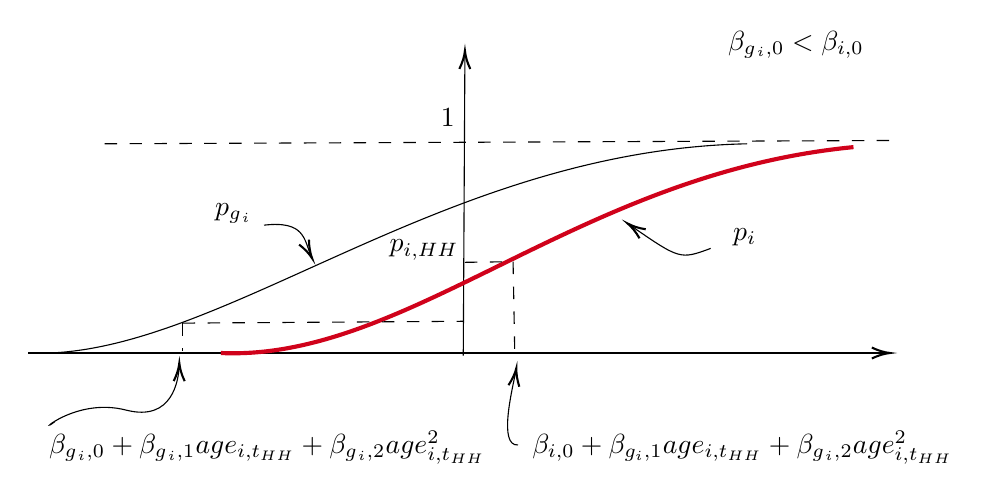
\begin{tikzpicture}[x=0.75pt,y=0.75pt,yscale=-1,xscale=1 , scale = 0.8]
%uncomment if require: \path (0,282); %set diagram left start at 0, and has height of 282

%Straight Lines [id:da01364414640014] 
\draw    (48,197) -- (565,197) ;
\draw [shift={(567,197)}, rotate = 180] [color={rgb, 255:red, 0; green, 0; blue, 0 }  ][line width=0.75]    (10.93,-3.29) .. controls (6.95,-1.4) and (3.31,-0.3) .. (0,0) .. controls (3.31,0.3) and (6.95,1.4) .. (10.93,3.29)   ;
%Straight Lines [id:da910788405565025] 
\draw    (310,198.5) -- (310.49,109.01) -- (310.99,17) ;
\draw [shift={(311,15)}, rotate = 90.31] [color={rgb, 255:red, 0; green, 0; blue, 0 }  ][line width=0.75]    (10.93,-3.29) .. controls (6.95,-1.4) and (3.31,-0.3) .. (0,0) .. controls (3.31,0.3) and (6.95,1.4) .. (10.93,3.29)   ;
%Straight Lines [id:da4713781086074158] 
\draw  [dash pattern={on 4.5pt off 4.5pt}]  (94,71) -- (569,69) ;
%Curve Lines [id:da12468730555344898] 
\draw    (48,197) .. controls (161,202) and (293.97,74.89) .. (481,71) ;
%Curve Lines [id:da5382648313464768] 
\draw [color={rgb, 255:red, 208; green, 2; blue, 27 }  ,draw opacity=1 ][line width=1.5]    (164,197) .. controls (277,202) and (379,89) .. (545,73) ;
%Straight Lines [id:da36157867825196655] 
\draw  [dash pattern={on 4.5pt off 4.5pt}]  (141,179) -- (141,196) ;
%Straight Lines [id:da8108377883655686] 
\draw  [dash pattern={on 4.5pt off 4.5pt}]  (340,142) -- (341,196.5) ;
%Curve Lines [id:da615268937283231] 
\draw    (459,134) .. controls (440.57,140.79)  .. (410.44,119.99) ;
%\draw    (459,134) .. controls (440.57,140.79) and (425.9,0.64) .. (410.44,119.99) ;
\draw [shift={(409,119)}, rotate = 34.51] [color={rgb, 255:red, 0; green, 0; blue, 0 }  ][line width=0.75]    (10.93,-3.29) .. controls (6.95,-1.4) and (3.31,-0.3) .. (0,0) .. controls (3.31,0.3) and (6.95,1.4) .. (10.93,3.29)   ;
%Curve Lines [id:da9903149181967108] 
\draw    (190,120) .. controls (214.57,117.17) and (214.14,128.62) .. (218.23,138.33) ;
\draw [shift={(219,140)}, rotate = 243.43] [color={rgb, 255:red, 0; green, 0; blue, 0 }  ][line width=0.75]    (10.93,-3.29) .. controls (6.95,-1.4) and (3.31,-0.3) .. (0,0) .. controls (3.31,0.3) and (6.95,1.4) .. (10.93,3.29)   ;
%Curve Lines [id:da19186794342848823] 
\draw    (342.97,252.38) .. controls (330.81,253.32) and (339.64,218.41) .. (341.68,207.83) ;
\draw [shift={(342,206)}, rotate = 97.95] [color={rgb, 255:red, 0; green, 0; blue, 0 }  ][line width=0.75]    (10.93,-3.29) .. controls (6.95,-1.4) and (3.31,-0.3) .. (0,0) .. controls (3.31,0.3) and (6.95,1.4) .. (10.93,3.29)   ;
%Curve Lines [id:da4976225910543626] 
\draw    (63.97,238.38) .. controls (51.97,247.38) and (75.97,223.38) .. (106.97,231.38) .. controls (135.02,238.62) and (138.51,213.1) .. (138.94,204.94) ;
\draw [shift={(139,203)}, rotate = 90.41] [color={rgb, 255:red, 0; green, 0; blue, 0 }  ][line width=0.75]    (10.93,-3.29) .. controls (6.95,-1.4) and (3.31,-0.3) .. (0,0) .. controls (3.31,0.3) and (6.95,1.4) .. (10.93,3.29)   ;
%Straight Lines [id:da10798771261096007] 
\draw  [dash pattern={on 4.5pt off 4.5pt}]  (141,179) -- (309.97,177.89) ;
%Straight Lines [id:da1934175682228103] 
\draw  [dash pattern={on 4.5pt off 4.5pt}]  (310.97,142.38) -- (340,142) ;

% Text Node
\draw (295,48) node [anchor=north west][inner sep=0.75pt]   [align=left] {1};
% Text Node
\draw (159,105.4) node [anchor=north west][inner sep=0.75pt]    {$p_{g}{}_{_{i}}$};
% Text Node
\draw (471,120.4) node [anchor=north west][inner sep=0.75pt]    {$p_{i}$};
% Text Node
\draw (59,242.4) node [anchor=north west][inner sep=0.75pt]    {$\beta _{g}{}_{_{i} ,0} +\beta _{g}{}_{_{i} ,1} age_{i,t_{HH}} +\beta _{g}{}_{_{i} ,2} age_{i,t_{HH}}^{2}$};
% Text Node
\draw (350,242.4) node [anchor=north west][inner sep=0.75pt]    {$\beta _{i,0} +\beta _{g_{i} ,1} age_{i,t_{HH}} +\beta _{g}{}_{_{i} ,2} age_{i,t_{HH}}^{2}$};
% Text Node
\draw (264,127.4) node [anchor=north west][inner sep=0.75pt]    {$p_{i,HH}$};
% Text Node
\draw (468,1.4) node [anchor=north west][inner sep=0.75pt]    {$\beta _{g}{}_{_{i} ,0} < \beta _{i,0}$};

\end{tikzpicture}

Once we have the probabilities of contributing, we simulate realizations of the contribution status as follows:
\begin{equation}
        contributes\_sim = \left \{ \begin{array}{ll}
         1 & if \ \ draw_1 \leq p_{i,e}  \\
         0 & otherwise 
            \end{array} \right .\\
\end{equation}
where $draw_1 \sim U[0,1]$.

(iii)  Imputing the probabilities of  evading contributions to social security and simulating the evasion status.

Let $pev_{i,t_{HH}}$ be  the probability that individual $i$ works conditional on not contributing (for short: probability of evading) in the year of the survey, estimated as explained in item \ref{prob_evading}. We compute the probabilities in other years $pev_{i,t}$ modifying ages accordingly:\footnote{For simplicity, we are omitting here time-invariant regressors. See panel\_active.do for the details. }
\begin{equation}
        pev_{i,t}= \left\{\begin{array}{ll}
            pev_{i,t_{HH}} & if \ t = t_{HH}, \\
            \frac{exp(\gamma_{i,0} +\gamma_{i,e} e + \gamma_{i,e2} e^2)}{1+ exp(\gamma_{i,0} +\gamma_{i,e} e + \gamma_{i,e2} e^2)},&  if  \ t \neq t_{HH} \ \ \& \ age_{i,t}=e. 
        \end{array} \right .
    \end{equation}

Using the probabilities of evading, we simulate the evasion status as follows:
\begin{equation}
        evades\_sim = \left \{ \begin{array}{ll}
         1 & if \ \ draw_2 \leq pev_{i,e} \ \& \ contributes\_sim = 0 \\
         0 & otherwise 
            \end{array} \right .\\
\end{equation}
where $draw_2 \sim U[0,1]$, independent of $draw_1$.



\item \label{item:pensions} \textbf{Estimating pensions}. For the year of the household survey, we take contributions and pensions exactly as the respondents reported to the survey. In this regard, we have no differences to other approaches, including the CEQ scenarios PGT and PDI. But the life-cycle approach also needs contributions and pensions in other years. The missing data is fundamentally different in the cases of (i) non-retired and (ii) retired individuals in the survey year.

(i) Individuals who were not retired in the household year. For these individuals we have the work histories simulated following the protocol described in item \ref{imputing-wh1}. In these cases, the remaining challenge is to compute pensions. We did it using the existing norms of the main Uruguayan pensions system, currently administered by the BPS-AFAP-BSE.\footnote{We do not describe the social security rules in this document, since it has already been described extensively in many publicly available documents \parencite{Forteza2012, Forteza2013a,  Saldain1995}.} As we already indicated, we proceed as if the whole population were covered by this system and the current rules had been present and were going to last forever. See the details in pensions.do. 

(ii) Individuals who were already retired in the household year. In these cases, we have a report of pensions, but we miss the contributions that gave place to the reported pension rights. So the challenge regarding these respondents of the survey is to impute work histories. We explain how we proceeded in the next item. 

    
\item \textbf{Imputing work histories to retired individuals}. \label{imputing-wh2} There is no direct information on labor income of individuals who were already retired when the household survey was gathered. We exploit the information contained in pensions reported to the survey to estimate work histories that are consistent with those pensions.

Using the information generated in step \ref{item:pensions}, we compute ratios of pensions to contributions for individuals who were working when the survey was gathered. With these ratios and the pensions reported to the survey, we compute labor income for the individuals who were retired in that year. 
The protocol is as follows:
\begin{enumerate}
    \item In each group $g_i$, we compute the average number of years of contribution of working-age individuals who are entitled to a pension according to the estimation explained in item \ref{item:pensions}. Let this variable be $tc_{g_i}$.
    \item We assume individuals retired as soon as they generated rights to receive a pension and contributed the last $tc_{g_i}$ years. Hence their histories of contribution are 
    \begin{equation}
        cont_{i,t}= \left \{
        \begin{array}{ll}
             1  & if \ age_{i,t}\in [ret\_age - tc_{g_i}, ret\_age - 1]  \\
             0 & otherwise 
        \end{array}
        \right .
    \end{equation}
    \item In each group $g_j$, we compute the expected replacement rate $rr_j$ of individuals who \textit{are not retired in the household survey}. Let $i\in g_j$ be a non-retired member of group $g_j$ and  $rr_i$ be her replacement rate, defined as follows
    \[ rr_i = pen_{i}/ali_i \]
    where
    $ali_i = {\sum_t y_{i,t}}/{\sum_t \mathbbm{1}(y_{i,t}>0)}$ is $i's$ average lifetime labor income.

    We compute group $j$ expected replacement rate as the median of the individual rates:
    \begin{equation} \label{eq:rr}
             rr_j = F_j^{-1}(0.5)
    \end{equation}
    where $F_j$ is the cdf of $rr_i, i\in g_j$.
    
  
 
    \item Using the replacement rates ($rr_j$) and the pensions reported to household survey ($pen_{i,t_{HH}}$), we compute the imputed average labor income  of the retiree $i$ ($iali_i$) as:
    \begin{equation} \label{eq:iali}
        iali_i = \frac{pen_{i,t_{HH}}}{rr_j} \ , \ \ i \in g_j 
    \end{equation}
    \item We compute the per-period labor income using the imputed average labor income ($iali_i$) and the age earnings profiles estimated with social security data ($g_{j,t}$):
     \begin{equation} \label{eq:liprofile}
     \begin{array}{ll}
          y_{i,t_0} &= \frac{iali_i \times \sum_t \mathbbm{1}(y_{i,t}>0) }{\sum_t \prod_{s=t_0+1}^t  (1+ g_{j,s})} \\
           y_{i,t}  &=  y_{i,t_0} \prod_{s=t_0+1}^t (1+ g_{j,t}) \ , \ \ t > t_0  
     \end{array}
    \end{equation}
    where $t_0$ is the first year in which individual $i$ works, and we have used that 
    \begin{equation} 
             iali_i  = \frac{\sum_t  y_{i,t}}{\sum_t \mathbbm{1}(y_{i,t}>0)}   
    \end{equation}
 
   
    \item Using the estimated contribution status and labor income we compute per-period contributions. 
\end{enumerate}
    See the details in panel\_active\_retired.do.
    
    \item \textbf{Estimating general taxes individuals pay to finance social security}\label{Estimating_taxes}. The PAYG programs are not necessarily fully financed with social security payroll contributions. If the program is in deficit, the government provides financial assistance using resources from general taxes. We compute the social security deficit as the difference between the sum of pensions paid and contributions collected.\footnote{The Uruguayan pension programs receive ear-marked taxes that are considered as ``own resources'' of the programs. These are not computed as ``financial assistance'' in the official accounting of social security. For our purposes, the distinction between ear-marked taxes and general taxes that funds financial assistance is irrelevant, so we compute these two concepts together.} We assume individuals contribute to the financing of the pensions program in proportion of their current labor income.\footnote{An alternative, probably more adequate, approximation would have been to assume that individuals contributions are proportional to their consumption. However this would have complicated estimations considerably because consumption can only be estimated once taxes have been computed. This alternative assumption would thus involve an iterative process.  } See the details in life\_cycle.do.
    
    \item \textbf{Evolution of households} \label{item:hh} 
    
     Decisions involving consumption and savings depend upon household aggregates, so we now move from individual to household analysis. These decisions depend on when the household was born and how long it is expected to last. Hence, we now present some simple assumptions about the evolution of households:
  \begin{enumerate}
    \item  We assume the household begins when (i) its oldest member turns 20 or (ii) in the year of the survey, if the oldest member was younger that year. We will refer to the oldest member as the ``head of household'' (hhh).\footnote{Notice this differs with the usage of the term in the Uruguayan survey, where respondents self identify the head of household. Our assumption helps to ascribe all individuals across their whole lifetime with existing households in 2017. The number of cases in which ours differs from the self reported identification of head of household is very small.} Formally, the starting year of family $j$ is 
    \begin{equation} \label{eq:hh\_t0}
        t_{j0} =   \left\{
             \begin{array}{ll}
                2017-(age_{hhh_j,2017}-20) & \text{if}  \ \ age_{hhh_j,2017} \geq 20 \\
                2017 & \text{otherwise}
            \end{array} \right.
    \end{equation}
     where $age_{hhh_j,2017}$ is the age of the head of household $j$ in 2017.  
      \item Members of the household. Let $J$ be the set of individuals $i$ in household $j$ in 2017. Head of households and adults  (individuals aged $\geq 20$ in 2017) remain with the same family until death. Children (individuals aged $<20$ in 2017 and not head of household), remain with the family until they turn $20$ or die. Formally, we define an indicator variable $\mathbbm{1}_{it}$ equal to 1 if the individual is in $t$ with the family he was in 2017 according to the household survey, provided he is alive in $t$: 
       \begin{equation} \label{eq:mofhh}
        \mathbbm{1}_{it}= \left \{
        \begin{array}{ll}
          1 & if \ \ i  = hhh_j \\
          1 & if \ \ age_{i,2017}\geq 20 \ \ \& \ t \geq t_{j0}   \\
          1 & if \ \ age_{i,2017}< 20
          \ \ \& \ t \geq t_{j0} 
          \ \ \&  \ age_{i,t}\in [0,19] \\
          0 & otherwise
        \end{array} \right .
    \end{equation}
      \item Children have no income, with the only exception of child income the family may have reported to the HH survey. Formally: the probability of working is set to ``almost'' zero, with a realization different from zero in 2017 if and only if the respondent reported positive child income. 
  \end{enumerate}

In computing household per capita income we consider (i) all members of household, (ii) split total household income equally and (iii) do not use equivalence scales \parencite[for other options, see][]{Blanchet2021} %AGREGAR REFERENCIAS SOBRE ESCALAS DE EQUIVALENCIA. 
  
  See the details in life\_cycle.do. 
    
    \item \textbf{\textbf{Estimating lifetime income and social security wealth}}. 
     
  The intertemporal budget constraints of household $j$ with and without the pensions program are
   \begin{equation} \label{eq:ibc2}
    \begin{array}{ll}
         \sum_{t=t_{j0}}^\infty \frac{\sum_{i\in J} \mathbbm{1}_{it} S_{it}}{(1+r(1-txc))^{t-t_{j0}}} c_{it}^p & = \bar y_j + ssw_j \\
         \sum_{t=t_{j0}}^\infty \frac{\sum_{i\in J} \mathbbm{1}_{it} S_{it}}{(1+r(1-txc))^{t-t_{j0}}} c_{it} & = \bar y_j   
    \end{array}
  \end{equation}
     where: 
     \begin{enumerate}
         \item $c_{it}^p$ and $c_{it}$ stand for individual $i$'s consumption with and without the pensions program, and
         \item $\bar y_j$ and $ssw_j$ stand for household $j's$ lifetime income and social security wealth and are computed as:
     \begin{equation} \label{eq:yj-ssw}
        \begin{array}{ll}
            \bar y_j = \sum_{t=t_{j0}}^\infty \sum_{i\in J} (y_{it}(1-txl)+dtr_{it}) \frac{S_{it}}{(1+r(1-txc))^{t-t_{j0}}} \\
            ssw_j = \sum_{t=t_{j0}}^\infty \sum_{i\in J} (p_{it}(1-txp)-\tau_{it}) \frac{S_{it}}{(1+r(1-txc))^{t-t_{j0}}} 
        \end{array}
    \end{equation}
    and $S_{it}$ is the survival probability of $i$ in year $t$, conditional on being alive (or unborn) in the household initial year $t_{j0}$.\footnote{As we mentioned before, in the present paper we are treating survivors pensions as if they had been generated by the beneficiary, i.e. as if they were old-age pensions. Accordingly, in equation (\ref{eq:yj-ssw}) and following equations we only consider longevity insurance. }
     \end{enumerate}
       
     
    As it is standard practice, in equation (\ref{eq:ibc2}) we are assuming that households consumption is constrained by their income ---they cannot leave unpaid debts, unless they die--- and exhausts households resources. The flows $c_{it}^p$ and $c_{it}$ in equation (\ref{eq:ibc2}) and  $y_{it}, dtr_{it}, p_{it}$ and $\tau_{it}$ in equation (\ref{eq:yj-ssw}) should be best thought as quantities of Arrow-Debreu securities paying one unit if individual $i$ is alive in $t$ and zero otherwise. Because of life insurance provided by the AD securities, individuals can equalize lifetime consumption and income without leaving unpaid debts or unintended bequests if they die.\footnote{Implicit behind equation (\ref{eq:ibc2}) is the assumption that there are no bequests. In item \ref{item:bequests}, we introduce intended bequests and show under which assumptions equation (\ref{eq:ibc2}) holds true despite of the existence of bequests.}
    
    See the details in life\_cycle.do.

    \item \textbf{Estimating per-period consumption and wealth, and non-labor income}
    
    Consumption can now be computed making some behavioral assumptions that provide the slope of the consumption paths. In our base case scenario we adopt the commonly used assumption of consumption smoothing: $c_{i,t}=\mathbbm{E}[c_{i,t+1}]$. We also assume all members of each family consume the same. With these assumptions, per capita consumption of family $j$, with and without the pensions program, fulfill:
     \begin{equation} \label{eq:ibc3}
    \begin{array}{ll}
         c_{j}^p  & = \frac{\bar y_j + ssw_j}{dmofhh_j}  \\
         c_{j}  & = \frac{\bar y_j }{dmofhh_j} 
    \end{array}
  \end{equation}
   where $dmofhh_j$ is the  discounted sum of the expected number of members of the household $j$ across the duration of the household, and is given by:
   \begin{equation} \label{eq:dmofhh}
   dmofhh_j = 
              \sum_{t=t_{j0}}^\infty \frac{\sum_{i\in J} \mathbbm{1}_{it} S_{it}}{(1+r(1-txc))^{t-t_{j0}}} 
   \end{equation}
    
    In the presence of the pensions program, the per-period budget constraints of household $j$ can be written as: 
\begin{equation} 	\label{eq:FBC1hh}
\begin{array}{ll}
       a_{i,t+1}^p = &\frac{S_{i,t}}{S_{i,t+1}}  [(1+ \rho_i ) a_{it}^p - p_{it}(1-txp) +  \tau_{it}]   \\
      a_{jt+1}^v  =&\frac{\sum_{i\in J} \mathbbm{1}_{i,t} S_{i,t}}{\sum_{i\in J} \mathbbm{1}_{i,t+1} S_{i,t+1}} [(1+r(1-txc)) a_{jt}^v + y_{it}(1-txl) \\
      &+dtr_{it} + p_{it}(1-txp) -  \tau_{it} - c_{j}^p] 
\end{array}
\end{equation}

where $a_{it}^p$ stands for member $i's$ pension assets in $t$, and $a_{jt}^v$ for family $j's$ per capita voluntary assets in $t$. The returns from social security $(\rho_i)$ are computed solving
\begin{equation} \label{eq:irr1} \sum_{t=1}^\infty S_{it} \frac{p_{it}(1-txp)-\tau_{it}}{(1+{\rho_i})^{t-1}}=0
\end{equation}	

In the absence of the pensions program, the per-period budget constraints of household $j$ can be written as:
\begin{equation} 	\label{eq:FBC4} 
      a_{jt+1}  = \frac{\sum_{i\in J} \mathbbm{1}_{i,t} S_{i,t}}{\sum_{i\in J} \mathbbm{1}_{i,t+1} S_{i,t+1}} [(1+r(1-txc)) a_{jt} + y_{it}(1-txl) +dtr_{it}  - c_{j}]
\end{equation}

We use equations (\ref{eq:FBC1hh}) and (\ref{eq:FBC4}) and assume that assets are zero in periods 0 and $T$ to compute per-period assets $a_{it}^p $, $a_{jt}^v$ and $a_{jt}$. As we explain in item \ref{item:bequests}, the assumptions $a_{i0}^p = a_{iT}^p = a_{j0}^v = a_{jT}^v=a_{j0}=a_{jT}=0$ do not necessarily imply that individuals do not leave bequests, but ony \textit{unintended} bequests.  

Assets in the per-period budget constraints should be thought as quantities of Arrow-Debreu securities. Specifically, in equation (\ref{eq:FBC1hh}), $a_{i,t}^p$  is individual $i$ holdings of contingent claims that pay one unit if the individual is alive in $t$ and zero otherwise, and have an actuarially fair price $S_{i,t}$ in $t_{j0}$. In equations (\ref{eq:FBC1hh}) and (\ref{eq:FBC4}), $a_{jt}^v$ and $a_{jt}$ are family $j$ holdings of securities that pay a fraction equal to the proportion of members of $j$ who are alive in $t$, and have prices $\sum_{i\in J} \mathbbm{1}_{i,t} S_{i,t}$  in $t_{j0}$. 

Notice that $a_{it}^p$ are not necessarily the financial assets held in the pensions program on behalf of individual $i$, but the implicit assets that represent $i's$ accrued pension rights (Forteza, 2017). 

While pension assets are determined at the individual level by the social security rules and individuals' work histories, voluntary savings are determined at the household level. So the system of equations (\ref{eq:FBC1hh}) generate as many series of pension assets as members the family has and only one series of voluntary savings.
	
Household $j's$ expected per-period disposable income, in the with (wp) and without (woutp) pensions scenarios can now be computed from equations (\ref{eq:FBC1hh}) and (\ref{eq:FBC4}) as:
\begin{equation} \label{eq:hh_income}
    \begin{array}{ll}
        \sum_{i\in J} \mathbbm{1}_{it}S_{i,t} [y_{it}(1-txl) +r(1-txc) a_{jt}^v+\rho_i a_{it}^p +dtr_{it}]  & wp   \\
         \sum_{i\in J} \mathbbm{1}_{it}S_{i,t}[y_{it}(1-txl)+r(1-txc) a_{jt} +dtr_{it} ] &  woutp 
    \end{array}
\end{equation}
Notice that $\rho_i a_{it}^p$ is already an ``after taxes'' concept, because taxes on pensions are incorporated in equation (\ref{eq:irr1}) where we compute the returns $\rho_i$.\footnote{Mandatory savings ``after taxes'' income can be written in the ``before taxes'' minus taxes format as follows: $\rho_i a_{it}^p = \rho^{bt}_i a_{it}^p - (\rho^{bt}_i - \rho_i)a_{it}^p $, where the before taxes rate of return is computed from $ \sum_{t=1}^\infty S_{it} \frac{p_{it}-\tau_{it}}{(1+{\rho^{bt}_i})^{t-1}}=0$. } 

Also notice that pensions and contributions are not part of family's income because these items cancel out in equations (\ref{eq:FBC1hh}). Indeed, adding expected assets of members of family $j$:
\begin{equation} 
\begin{array}{ll}
      \sum_{i\in J} \mathbbm{1}_{i,t+1} S_{i,t+1} a_{i,t+1}^p = &\sum_{i\in J} \mathbbm{1}_{i,t} S_{i,t} [(1+ \rho_i ) a_{it}^p \\
      &- p_{it}(1-txp) +  \tau_{it}]   \\
      \sum_{i\in J} \mathbbm{1}_{i,t+1} S_{i,t+1} a_{j,t+1}^v  =&\sum_{i\in J} \mathbbm{1}_{i,t} S_{i,t} [(1+r(1-txc)) a_{j,t}^v \\
      &+ y_{i,t}(1-txl) +dtr_{it}\\
      &+ p_{it}(1-txp) -  \tau_{it} - c_{j}^p] 
\end{array}
\end{equation}
Adding mandatory and voluntary assets and reorganizing terms:
\begin{equation} 	\label{eq:FBC3}
    \begin{array}{ll}
         a_{j,t+1}^{ss} - a_{j,t}^{ss} = &  \sum_{i\in J} \mathbbm{1}_{i,t} S_{i,t} [y_{i,t}(1-txl)+dtr_{it} \\
    &+ r(1-txc) a_{j,t}^v +\rho_i a_{i,t}^p - c_{j}^p]
    \end{array} 
\end{equation}
where $a_{j,t}^{ss}$ stands for total expected assets in the presence of social security and is computed as:
\[a_{j,t}^{ss} = \sum_{i\in J} \mathbbm{1}_{i,t} S_{i,t}(a_{it}^p + a_{j,t}^v)  \]
The concept of income presented in the first raw of equation (\ref{eq:hh_income}) shows up in the right hand side of equation (\ref{eq:FBC3}). Pensions and contributions to the pension system impact on income through returns from assets and only if (i) they force an accumulation of assets different from what families would voluntary have saved without the program or (ii) the returns from social security assets are different from market returns. Otherwise they have no effect. In particular, an individual accounts system has no material impact on individuals incomes, unless it forces mandatory savings above voluntary savings without pensions. 

In the case of individuals who contribute some periods but do not access a pension, the income from mandatory savings tends to minus the sum of contributions and taxes paid to finance pensions, augmented by the mortality bonus. Notice that the internal rate of return tends to $-1$ as pensions tend to zero from above: $lim_{p_k \to 0} \rho_k = -1$.\footnote{We use here that the first and last terms of pension cash flows are negative and non-negative numbers, respectively.} Substituting in the first row of equations (\ref{eq:FBC1hh}), we have that income from mandatory savings of individual $k$ whose pension tends to zero is:   
 \begin{equation} \label{eq:income_no_access}
     \lim_{p_k \to 0} \rho_k a_{k,t}^p  = - \frac{ S_{i,t-1}}{S_{i,t}}  \tau_{k,t-1}
 \end{equation}
 
In this sense, contributions become a pure tax when individuals do not fulfill the vesting period conditions required to receive a pension. 

Similar arguments lead to the concept of income in the absence of a pension program presented in the second raw of equations (\ref{eq:hh_income}). 

Our empirical analysis of the distribution of 2017 income is an analysis of realized ---as opposed to expected--- income in a particular year. Among other things, this implies that individuals in our database are alive in 2017. So, to compute 2017 income concepts we substitute $S_{i,t}=1, \forall i \ \& \ t\leq 2017$,  in equations (\ref{eq:hh_income}) and (\ref{eq:income_no_access}).

See the details in life\_cycle.do.

\item \textbf{Calibrating income from wealth.} \label{item:bequests}

Income from wealth computed using equations (\ref{eq:FBC1hh}) and (\ref{eq:FBC4}) and a no bequest assumption do not necessarily match reported data. In order to replicate reported capital income, we avoid the no-bequest assumption and rather assume that individuals receive and leave bequests \parencite[for a similar argument, see among others][]{Fullerton1991, Kotlikoff1981}.  

We specifically assume that bequests received and left are equal in present value.   Let $b_{i,t_i}$ be the bequest the individual $i$ receives in $t_i$ and $b_{i,t}, t \geq t_i,$ the bequest the individual leaves in $t$ if he dies in that period. The assumption is that 
\begin{equation}  \label{eq:bequest}
    b_{i,t+1}=(1+r(1-txc))b_{i,t} , \ t \geq t_i
\end{equation}

So the individual is saving the bequest and leaving it for the descendants. This very simple assumption is consistent with a steady state in the sense that individuals leave the same they receive. 

Notice that these assets and the associated income do not modify the budget constraints (\ref{eq:FBC1hh}) and (\ref{eq:FBC4}) and the computations based on them, but total assets and per-period income from wealth are larger in the presence of bequests because the bequest assets must be added. 

Household \textit{j's} expected income is given by equations (\ref{eq:hh_income}), under the no bequest assumption, and (\ref{eq:hh_income2}), under the assumption that there are bequests that follow the rule (\ref{eq:bequest}).       
\begin{equation} \label{eq:hh_income2}
    \begin{array}{ll}
        \sum_{i\in J} \mathbbm{1}_{it}S_{i,t} [y_{it}(1-txl)+r(1-txc) (a_{jt}^v +b_{i,t})+ \rho_i a_{it}^p +dtr_{it} ]  & wp  \\
         \sum_{i\in J} \mathbbm{1}_{it}S_{i,t}[y_{it}(1-txl) +r(1-txc) (a_{jt}+b_{i,t}) +dtr_{it}] &  woutp
    \end{array}
\end{equation}

We compute intended bequests equalizing reported and simulated capital income of the household in the scenario with pensions. Let $r(1-txc)k_{j,t_{HH}}$ be household j capital income reported to the household survey in year $t_{HH}$. All members of the household are alive in the year of the survey so we equalize reported and simulated capital income conditional on individuals being alive:   $r(1-txc)k_{j,t_{HH}}= \sum_{i\in J} \mathbbm{1}_{i,t_{HH}} r(1-txc) [a_{jt}^v+b_{i,t_{HH}}]$. We compute families intended bequests in the year of the household as
\begin{equation} \label{eq:income-bequests}
    \sum_{i\in J} \mathbbm{1}_{i,t_{HH}} r(1-txc) b_{i,t_{HH}} = r(1-txc)k_{j,t_{HH}}- \sum_{i\in J} \mathbbm{1}_{i,t_{HH}} r(1-txc) a_{j,t_{HH}}^v
\end{equation}
 
Finally, we compute realized after-tax capital income in the counterfactual scenario without pensions in the year of the survey as %$\sum_{i\in J} \mathbbm{1}_{i,t_{HH}} r (a_{j,t_{HH}}+b_{i,t_{HH}})$. 
\begin{equation} \label{eq:capital-income-NSS}
    \sum_{i\in J} \mathbbm{1}_{i,t_{HH}} r(1-txc) (a_{j,t_{HH}}+b_{i,t_{HH}})
\end{equation}

 
  
\item \textbf{Estimating distribution of income with and without pensions.} We finally compare income distribution in the year of the household survey with and without the pensions program. To this end, we compute the Gini indexes of these two measures of income. 
%Kakwani and Reynolds-Smolensky indexes... DESARROLLAR

See the details in inequality\_indexes.do.

\end{enumerate}

\begin{comment}
ATENCION: POR AHORA, NO ESTOY PONIENDO ALGUNAS COSAS:
\begin{itemize}

    \item CEQ. ALGUNOS DO FILE TRAEN O REPRODUCEN RESULTADOS DE ESTIMACIONES CEQ. NO ESTOY SEGURO TODAVIA SI CORRESPONDE EXPLICARLAS AQUI O NOS LIMITAMOS A REMITIR A LAS REFERENCIAS QUE CORRESPONDA. SI ENTENDI BIEN, DIEGO Y MARISA YA TIENEN ESTIMACIONES CEQ CON ECH 2017. PODRIAMOS SIMPLEMENTE DECIR QUE TOMAMOS ESAS ESTIMACIONES PARA COMPARAR CON LAS QUE SE OBTIENEN CON EL LIFE-CYCLE APPROACH Y REMITIR AL LECTOR AL O LOS ARTICULOS DE USTEDES (diego y marisa). 
\end{itemize}

\end{comment}


\end{document}